%% This is file `elsarticle-template-2-harv.tex',
%%
%% Copyright 2009 Elsevier Ltd
%%
%% This file is part of the 'Elsarticle Bundle'.
%% ---------------------------------------------
%%
%% It may be distributed under the conditions of the LaTeX Project Public
%% License, either version 1.2 of this license or (at your option) any
%% later version.  The latest version of this license is in
%%    http://www.latex-project.org/lppl.txt
%% and version 1.2 or later is part of all distributions of LaTeX
%% version 1999/12/01 or later.
%%
%% The list of all files belonging to the 'Elsarticle Bundle' is
%% given in the file `manifest.txt'.
%%
%% Template article for Elsevier's document class `elsarticle'
%% with harvard style bibliographic references
%%
%% $Id: elsarticle-template-2-harv.tex 155 2009-10-08 05:35:05Z rishi $
%% $URL: http://lenova.river-valley.com/svn/elsbst/trunk/elsarticle-template-2-harv.tex $
%%

%%\documentclass[preprint,authoryear,12pt]{elsarticle}

%% Use the option review to obtain double line spacing
%% \documentclass[authoryear,preprint,review,12pt]{elsarticle}

%% Use the options 1p,twocolumn; 3p; 3p,twocolumn; 5p; or 5p,twocolumn
%% for a journal layout:

%% Astronomy & Computing uses 5p
%% \documentclass[final,authoryear,5p,times]{elsarticle}
\documentclass[final,authoryear,5p,times,twocolumn]{elsarticle}

%% if you use PostScript figures in your article
%% use the graphics package for simple commands
%% \usepackage{graphics}
%% or use the graphicx package for more complicated commands
\usepackage{graphicx}
%% or use the epsfig package if you prefer to use the old commands
%% \usepackage{epsfig}

%% The amssymb package provides various useful mathematical symbols
\usepackage{amssymb}
%% The amsthm package provides extended theorem environments
%% \usepackage{amsthm}

\usepackage[pdftex,pdfpagemode={UseOutlines},bookmarks,bookmarksopen,colorlinks,linkcolor={blue},citecolor={green},urlcolor={red}]{hyperref}
\usepackage{hypernat}

%% The lineno packages adds line numbers. Start line numbering with
%% \begin{linenumbers}, end it with \end{linenumbers}. Or switch it on
%% for the whole article with \linenumbers after \end{frontmatter}.
%% \usepackage{lineno}

%% natbib.sty is loaded by default. However, natbib options can be
%% provided with \biboptions{...} command. Following options are
%% valid:

%%   round  -  round parentheses are used (default)
%%   square -  square brackets are used   [option]
%%   curly  -  curly braces are used      {option}
%%   angle  -  angle brackets are used    <option>
%%   semicolon  -  multiple citations separated by semi-colon (default)
%%   colon  - same as semicolon, an earlier confusion
%%   comma  -  separated by comma
%%   authoryear - selects author-year citations (default)
%%   numbers-  selects numerical citations
%%   super  -  numerical citations as superscripts
%%   sort   -  sorts multiple citations according to order in ref. list
%%   sort&compress   -  like sort, but also compresses numerical citations
%%   compress - compresses without sorting
%%   longnamesfirst  -  makes first citation full author list
%%
%% \biboptions{longnamesfirst,comma}

% \biboptions{}

\journal{Astronomy \& Computing}

\begin{document}

\begin{frontmatter}

%% Title, authors and addresses

%% use the tnoteref command within \title for footnotes;
%% use the tnotetext command for the associated footnote;
%% use the fnref command within \author or \address for footnotes;
%% use the fntext command for the associated footnote;
%% use the corref command within \author for corresponding author footnotes;
%% use the cortext command for the associated footnote;
%% use the ead command for the email address,
%% and the form \ead[url] for the home page:
%%
%% \title{Title\tnoteref{label1}}
%% \tnotetext[label1]{}
%% \author{Name\corref{cor1}\fnref{label2}}
%% \ead{email address}
%% \ead[url]{home page}
%% \fntext[label2]{}
%% \cortext[cor1]{}
%% \address{Address\fnref{label3}}
%% \fntext[label3]{}

\title{Automated reduction of submillimetre single-dish heterodyne
  data from the James Clerk Maxwell Telescope using ORAC-DR}

%% use optional labels to link authors explicitly to addresses:
%% \author[label1,label2]{<author name>}
%% \address[label1]{<address>}
%% \address[label2]{<address>}

\author[jac,cornell]{Tim Jenness\corref{cor1}}
\ead{tjenness@cornell.edu}
\author[jac]{Malcolm J.\ Currie}
\ead{m.currie@jach.hawaii.edu}
\author[jac]{Remo P.\ J.\ Tilanus\fnref{rpt}}
\author[jac]{Brad Cavanagh}
\author[jac]{David S. Berry}
\author[jac]{Jamie Leech\fnref{jxl}}
\author[jac]{Luca Rizzi\fnref{lr}}

\cortext[cor1]{Corresponding author}
\fntext[rpt]{Present address: Leiden Observatory, PO Box 9513, 2300 RA
  Leiden, The Netherlands}
\fntext[jxl]{Present address: Department of Physics, University of
  Oxford, Denys Wilkinson Building, Keble Road, Oxford, OX1 3RH, UK}
\fntext[lr]{Present address: W.\ M.\ Keck Observatory, 65-1120 Mamalahoa Hwy, Kamuela,
  HI 96743, USA}

\address[jac]{Joint Astronomy Centre, 660 N.\ A`oh\=ok\=u Place, Hilo, HI
  96720, USA}
\address[cornell]{Department of Astronomy, Cornell University, Ithaca,
  NY 14853, USA}

\begin{abstract}
%% Text of abstract

With the advent of modern multi-receptor heterodyne instruments that
can result in observations generating thousands of spectra per minute it is
no longer feasible to reduce these data as individual spectra. This
paper describes how baselined, mosaicked data cubes can be created by
an automated pipeline in a reliable manner, including detection of bad
spectra, removal of transient effects and creation of high fidelity
moment maps.

\end{abstract}

\begin{keyword}
%% keywords here, in the form: keyword \sep keyword

%% MSC codes here, in the form: \MSC code \sep code
%% or \MSC[2008] code \sep code (2000 is the default)

submillimeter astronomy \sep
methods: data analysis \sep
pipelines \sep
techniques: spectroscopic \sep
techniques: image processing \sep
James Clerk Maxwell Telescope

\end{keyword}

\end{frontmatter}

% \linenumbers

%% Journal abbreviations
\newcommand{\mnras}{Mon Not R Astron Soc}
\newcommand{\aap}{Astron Astrophys}
\newcommand{\pasp}{Pub Astron Soc Pacific}
\newcommand{\apj}{Astrophys J}
\newcommand{\apjs}{Astrophys J Supp}
\newcommand{\qjras}{Quart J R Astron Soc}
\newcommand{\an}{Astron.\ Nach.}
\newcommand{\ijimw}{Int.\ J.\ Infrared \& Millimeter Waves}
\newcommand{\procspie}{Proc.\ SPIE}
\newcommand{\aspconf}{ASP Conf. Ser.}

%% Applications
\newcommand{\makecube}{\textsc{Makecube}}

%% main text
\section{Introduction}
\label{sec:intro}

As heterodyne receivers have progressed from single-receptor
instruments
\citep{1992IJIMW..13.1487P,1992IJIMW..13..647D,1992IJIMW..13.1827C} to
small focal plane arrays
\citep{2003SPIE.4855..322G,2004A&A...423.1171S} to 16 element arrays
such as HARP at JCMT \citep{2009MNRAS.399.1026B}, and beyond
\citep{2012SPIE.8452E..04K}, and correlators have improved such that
we can easily obtain spectra at 10\,Hz with 8192 channels, data rates
have increased substantially such that it is now common-place to take
a short observation resulting in thousands of spectra. This is only
going to become more challenging with the advent of instruments with
64,000 channels and dual-waveband arrays each of which consist of 128
detectors,  such as the CHAI instrument proposed for CCAT
\citep{2009ASPC..417..113R,GoldsmithCHAI2012,P10_adassxxiii}.

In submillimeter astronomy data reductions packages such as
\htmladdnormallinkfoot{CLASS}{http://www.iram.fr/IRAMFR/GILDAS}
(ascl:1305.010) and
SPECX \citep{SPECX} were developed that worked well with
single-receptor instruments. Scripting interfaces and tools for
curating collections of spectra were insufficient as the data rates
increased and data pipelines \citep[e.g.,][]{1995ASPC...75..117W} and
algorithms that work on the full data set
\citep[e.g.,][]{2002ASPC..278..329M} were suggested. The ACSIS data
reduction system \citep{2000ASPC..216..502L,2000SPIE.4015..114H},
delivered to the JCMT in 2005, aimed to deal with the data rate issues
by providing a pipeline that sent the calibrated spectra, with
optional baselining, to a component that would place the spectra in to
a data cube. Although it was possible to store the raw data in CASA
(ascl:1107.013) measurement sets \citep{2012ASPC..461..849P}\footnote{At the time this
  was being developed CASA was known as AIPS++
  \citep{2004ASPC..314..468M}}, the data cube was the product that was
archived and taken away by the astronomer for further analysis. This
strategy was forced on us given the computer resources available when
ACSIS was being designed and developed and was known to have risks
associated with it. Coadding spectra into the cube allowed for
impressive ``data compression'' for stare and jiggle observing modes
although the gains were much less in scanning observing modes. There
were many downsides though. The observing system required that the
cube parameters be specified and initially it was felt that the
observer should select the parameters in the Observing Tool
\citep{2002ASPC..281..453F}. It was also necessary that the observer
specify the baseline regions and any frequency binning required. The
gridding and the frequency binning were irreversible and the observer
needed to ensure they did not make a mistake. Additionally, baselining
with anything other than a DC offset was also problematic as the fit
parameters for every spectrum were not stored and so could not be
reversed. The burden placed on the observer having to specify
everything, whilst simultaneously not making a mistake, was not
acceptable and by 2006 we realised that computers were fast enough and
storage large enough to be able to write the calibrated spectra
directly to disk and defer further data reduction to a pipeline.

\section{Heterodyne Data Reduction Pipeline}

It was decided that data reduction recipes would be written for the
existing ORAC-DR pipeline infrastructure in use at JCMT
\citep{2011tfa..confE..42J,2008AN....329..295C} with key requirements
that the output data cube should be specified from the telescope
pointing information and the location of each receptor on the sky, and
that baseline regions should be determined automatically by examining
the spectra as an ensemble. Furthermore, as progress was made on the
pipeline we additionally realised that we should also be able to
detect bad spectra and remove them from the coadd as well as doing
quality assurance (QA) tests (see \S\,\ref{sec:qa}). The latter were
critical for the JCMT Legacy Survey projects
\citep{2007PASP..119..855W,2009ApJ...693.1736W,2007PASP..119..102P}
who wanted to ensure they received data of consistent quality.

The JCMT heterodyne pipeline has two operating modes. The default
behaviour is for the pipeline to generate the best possible data
products without regard to efficiency. This is generally what is
required by scientists at their institutions and the mode we run in at
the JCMT Science Archive
\citep{2008ASPC..394..135G,2008ASPC..394..565J}. The other mode is a
cut-down version of the recipes that runs at the JCMT itself during
observing. This pipeline has constrained timing requirements and can
not perform many of the advanced processing features provided by the
main pipeline. It's role is to provide simple quality assurance
information and basic coadds to the observer and it will not be
discussed further in this paper.

\subsection{Determining Cube Parameters}
\label{sec:makecube}

Once we decided that we would not require that a PI specifies the
output pixel grid of the data cube in advance, it became clear that we
would have to provide software that would automatically determine the
pixel grid from the data itself. In the SMURF package data cubes are
created from calibrated spectra using the \makecube\
command. \makecube\ can be given an externally specified grid but also
has an \texttt{autogrid} option that leaves optimal grid determination
to the application itself.

Autogrid first projects the supplied sky positions into pixel
positions using an arbitrary tangent plane projection that has
1~arcmin square pixels with North upwards and the target position
(or the first supplied sky position if no target position is
available) at pixel (1,1).

It then projects each of these pixel positions onto a straight line
passing through pixel (1,1) at an angle, $\theta$, to North (see
Fig.~\ref{fig:autogrid}). This line is divided up into sections of
length 1~arcmin, and a histogram formed of the number of projected
positions that fall in each section. The amplitude and wavelength of
any periodicity in this histogram is found by looking at the
auto-correlation of the histogram (the amplitude is the
auto-correlation at zero shift, and the wavelength is the shift at the
first significant peak in the auto-correlation function).

\begin{figure}
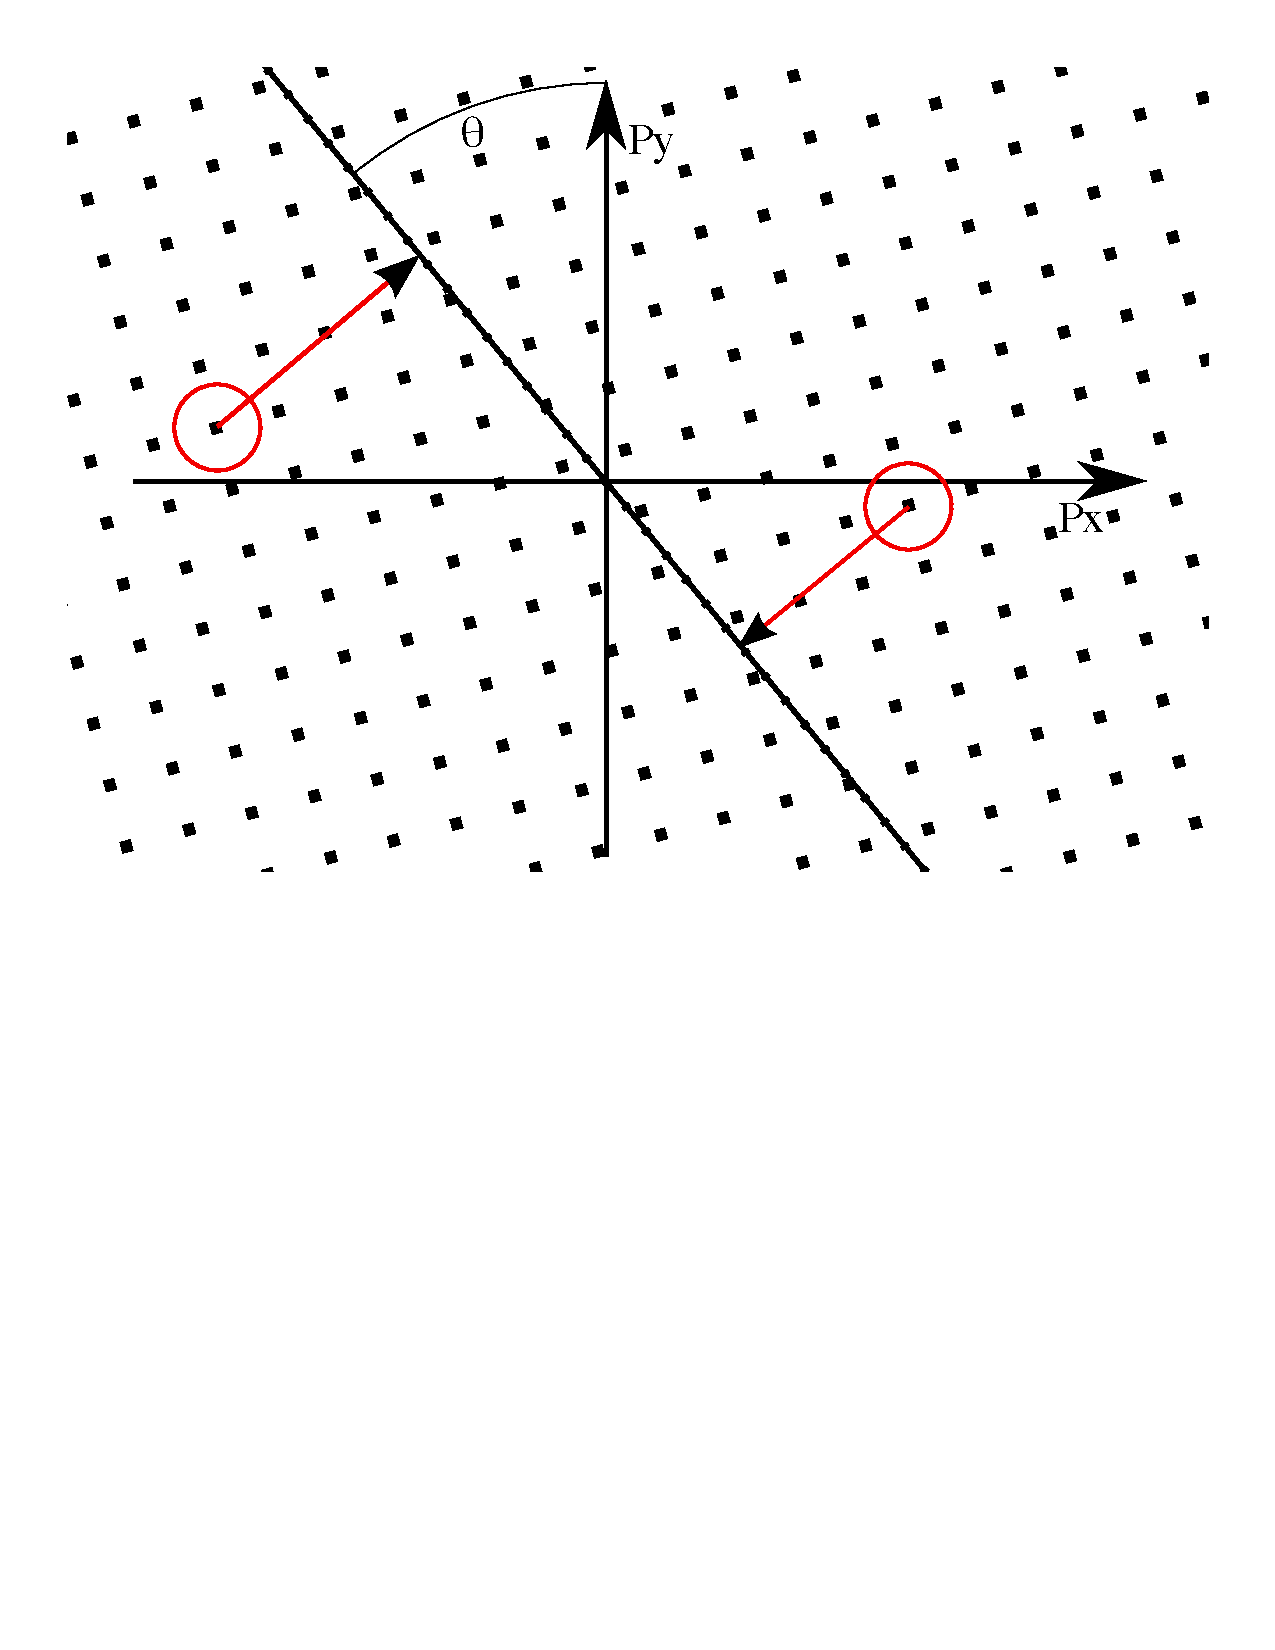
\includegraphics[width=0.48\textwidth]{autogrid}
\caption{The Autogrid algorithm works by projecting each spectrum
  position onto a straight line at an arbitrary angle $\theta$, and then
  forming a histogram of the number of samples at each point along
  this line. At the optimal value of $\theta$, the projected positions
  line up, giving strong periodicity in the histogram.}
\label{fig:autogrid}
\end{figure}

This is repeated for many different line orientations in order to find
the value of $\theta$ (line orientation) that gives the strongest
periodicity in the histogram. This orientation is used as the
direction for the X pixel axis in the final grid. The corresponding
wavelength is used as the pixel spacing on the X axis. The wavelength
of the periodicity perpendicular to this direction is then found and
used as the pixel spacing on the Y axis.

Finally, we shift the reference pixel coordinates by up to one pixel
on each axis in order to minimise the sum of the squared distances
from each pixel projected sample position to the nearest pixel centre.

If the positions do not form a regular grid, an option is available to
create a 1-dimensional list of spectra in which the position of each
spectrum is recorded explicitly in a table using the FITS-WCS
\texttt{-TAB} algorithm \citep{2006A&A...446..747G}.

The output spectrum at each position on the grid is formed by
averaging the nearby input spectra. Various averaging schemes are
available, the simplest being to place each input spectrum entirely
into the nearest output pixel. Other schemes allow a 2-dimensional
kernel to be used to spread each input spectrum out over a range of
output pixels. Available kernels are those supported by the AST
library \citep{SUN211,2012ASPC..461..825B} and include a simple
bi-linear division between the four nearest neighbours, a Gaussian
kernel, and various flavours of kernels based on a sinc function.

When using nearest neighbour resampling there are multiple ways to
determine how bad pixels are propagated from input spectra into the
output cube. The \texttt{AND} scheme uses all input data (thus
reducing the noise in the output) and also minimises the number of bad
pixels in the output. However, the memory requirements of the
\texttt{AND} scheme can be excessive. For this reason, two other
schemes, \texttt{FIRST} and \texttt{OR}, are provided which greatly
reduce the memory requirements, at the expense either of introducing
more bad pixels into the output (\texttt{OR}) or producing higher
output noise levels (\texttt{FIRST}).

\begin{description}
\item[\texttt{FIRST}] The bad-pixel mask in each output spectrum is
  inherited from the first input spectrum that contributes to the
  output spectrum. Any subsequent input spectra that contribute to the
  same output spectrum but which have a different bad-pixel mask are
  ignored. So an output pixel will be bad if and only if the
  corresponding pixel in the first input NDF that contributes to it is
  bad. Since this scheme ignores entire input spectra if they do not
  conform to the expected bad-pixel mask, the noise in the output can
  be higher than using the other schemes. However, this scheme has the
  benefit of using much less memory than the \texttt{AND} scheme, and
  will in general produce fewer bad pixels in the output than the
  \texttt{OR} scheme.

\item[\texttt{OR}] The bad pixel mask in each output spectrum is the
  union (logical OR) of the bad pixel masks for all input spectra that
  contribute to the output spectrum. So an output pixel will be bad if
  any of the input pixels that contribute to it are bad.  This scheme
  will in general produce more bad output pixels than the
  \texttt{FIRST} scheme, but the non-bad output pixels will have a
  lower noise because, unlike \texttt{FIRST}, all the contributing
  input data are coadded to produce the good output pixels. Like
  \texttt{FIRST}, this scheme uses much less memory than \texttt{AND}.

\item[\texttt{ AND}] The bad pixel mask for each output spectrum is
  the intersection (logical AND) of the bad pixel masks for all input
  spectra that contribute to the output spectrum. So an output pixel
  will be bad only if all the input pixels that contribute to it are
  bad. This scheme will produce fewer bad output pixels and will also
  give lower output noise levels than \texttt{FIRST} or \texttt{OR},
  but at the expense of much greater memory requirements.

\end{description}

The pipeline processing defaults to using the \texttt{AND} scheme but
can be overridden if speed or memory are an issue.

One complication is that the data cube for a large area survey is
potentially extremely large and many software package do not support
data arrays with more than $2^{32}$ pixels. We overcome this by
supporting the ability for the output cube from \textsc{makecube} to
be split into tiles. These tiles share projection parameters and can
be recombined without further resampling if required. For pixel
spreading techniques that are susceptible to edge effects care is
taken to ensure that sufficient border is included in the tiles such
that the values in the output would be identical to those resulting
from a single output data cube. The border region is flagged in an
associated bit mask to ensure that it can be disabled during further
mosaicking or combination steps as the data in the border region will
have edge effects and is duplicating data found in other tiles.

\subsection{Sub-band merging}

In hybrid modes the correlator is configured to use multiple
hardware subsystems to process parts of the required bandwidth so
that they can be combined in the data reduction. The correlator is
usually configured such that the individual spectra overlap and also
have channels that are aligned to within a few per cent of a pixel.

The data acqusition system does not combine the subbands and so this
must be done by the pipeline. If the pipeline determines that it is
dealing with a hybrid mode observation the merging is done in
bulk. First the spectra are sorted by time (the ACSIS acquisition
computer does not guarantee that spectra will be written to files in
time order), then the overlap region is determined and the noisy ends
are trimmed before they are combined. The spectra can optionally have
their DC level adjusted before combining.

\begin{figure}
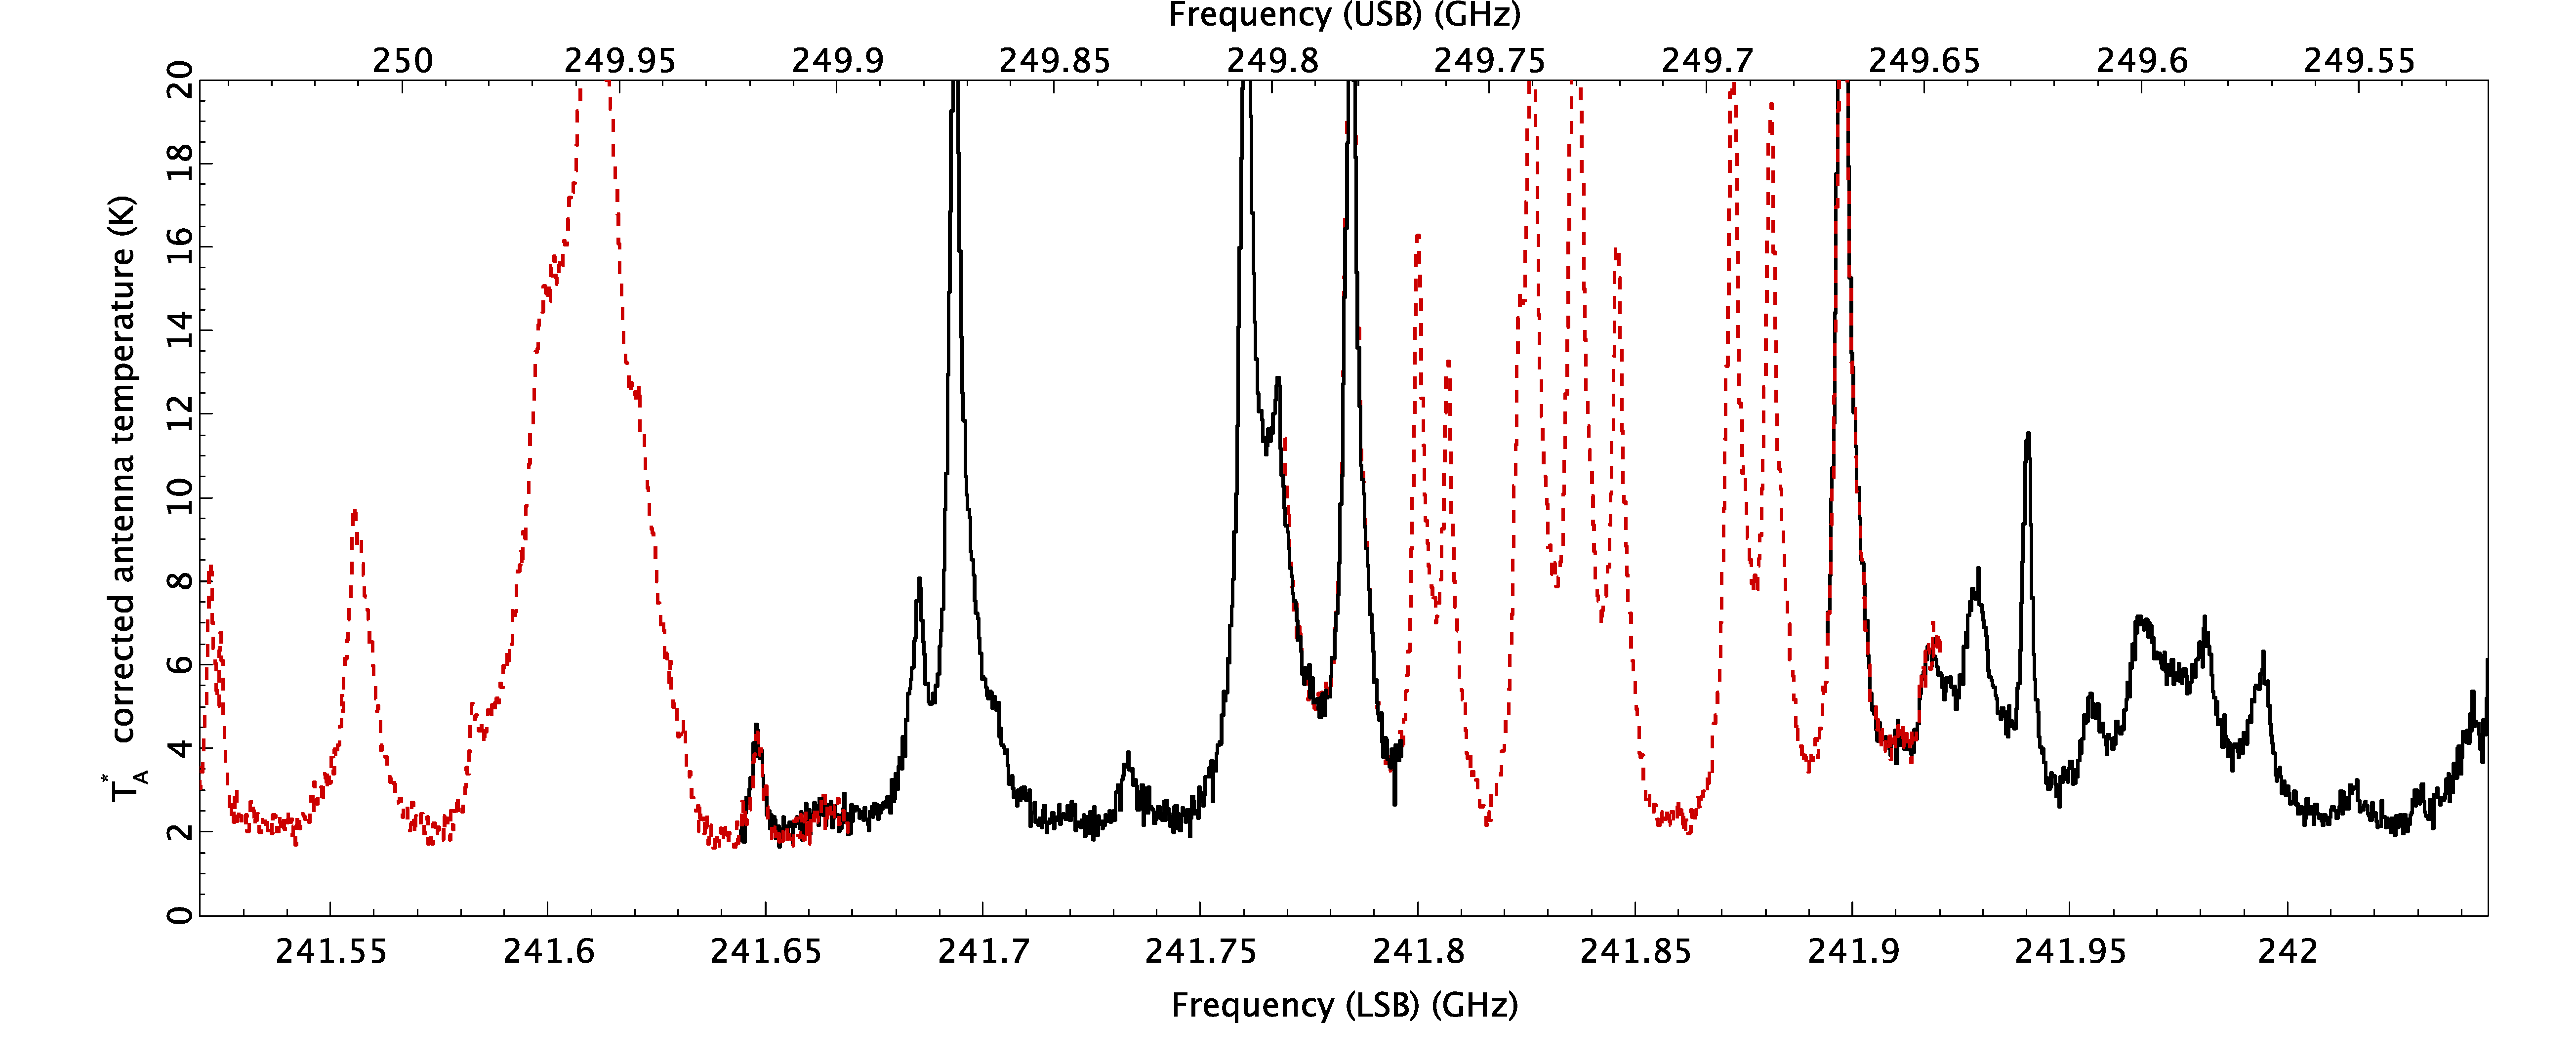
\includegraphics[width=90mm]{hybrid}
\caption{A hybrid spectrum from an observation in Orion of multiple
  methanol transitions. The frequency scale is for the kinematic local
  standard of rest and the observations were taken with a rest
  frequency of 241.791\,GHz. These data were taken on 1998 December 20
  as part of project M98BA3I.}
\label{fig:hybrid}
\end{figure}

Fig.\ \ref{fig:hybrid} shows an example hybrid spectrum consisting of
4 overlapping subbands from observations of methanol in Orion. In this
example correcting for any DC offset is complicated by the lack of
baseline region.

\subsection{Automated Baseline Removal}

\begin{figure}
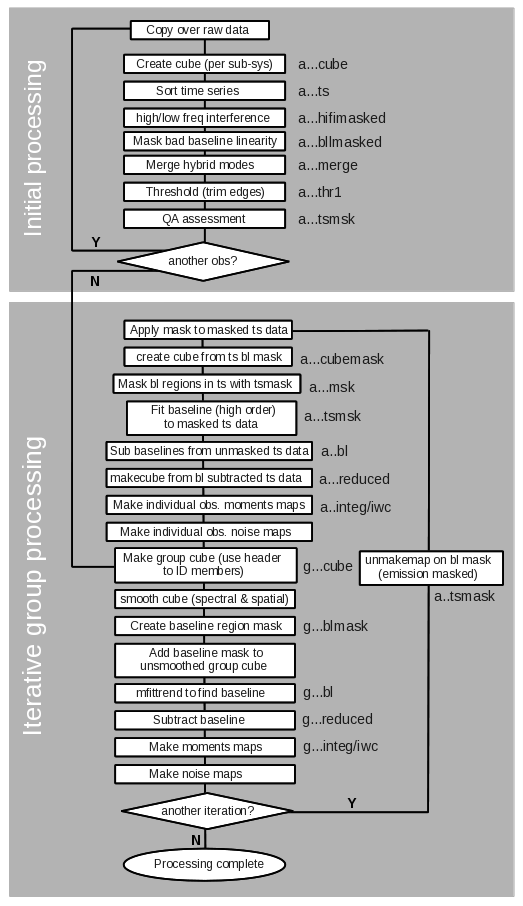
\includegraphics[width=90mm]{flowchart}
\caption{Flow chart of the pipeline recipe, including the initial step
  where individual observations are analysed. \emph{QA} here indicates
a quality assurance test (see \S\,\ref{sec:qa})}
\label{fig:flowchart}
\end{figure}

Fig.\ \ref{fig:flowchart} shows the key steps in the automated
baseline removal algorithm. The initial phase involves the creation of
cubes from individual observations and a basic quality assurance test
to remove obviously problematic spectra. Once this is completed a cube
is created from all the observations. This cube will have baseline
offsets and an estimate for these offsets has to be calculated before
the advanced baseline processing can be performed. This is done by
applying a tophat smooth in three dimensions to spread the line
emission and baseline errors across multiple spatial positions. The
Starlink KAPPA task \textsc{mfittrend} then is used to calculate a
first order baseline fit for each spectrum in the data cube
independently. The baseline region is estimated by... \emph{MJC to
  write a description of AUTO mode in MFITTREND}.

Once \textsc{mfittrend} has calculated and removed a first pass at the
baseline a mask is written out containing the baseline regions of the
smoothed data cube. This mask is applied to the original
unsmoothed data cube resulting in a cube consisting solely of
baselines. \textsc{mfittrend} is then used again but this time fitting
the entire (masked) spectrum, fitting a linear baseline to each
spectrum in turn. The baselines are then finally subtracted from the
original data cube.

Now that a good estimate for a baseline has been subtracted the data
cube can be analysed using more holistic approaches that can use
information from source features in the molecular cloud or galaxy that
span multiple spatial pixels. A clump-finding algorithm can be used to
accurately distinguish the line features from baseline regions which
can maximize optimize the baseline subtraction and aid in moment map
creation (see \S \ref{sec:moment}). The Starlink \textsc{cupid}
\citep{2007ASPC..376..425B} application contains a number of
clump-finding algorithms that work in three dimensions. The choice of
a particular algorithm is not critical and either Fellwalker or
Clumpfind \citep{1994ApJ...428..693W} can be used.

With an accurate knowledge of the line emission regions in the data
there is now the option of applying this mask to the raw data. The
SMURF \textsc{unmakecube} task is used for this. This application
reads a raw time series cube and generates a new time series by
calculating the position of each spectrum, looking up this position in
the group data cube mask and writing the emission-masked spectrum to
an output time-series cube. This time-series cube can then be used to
mask the original time-series allowing the baseline to be fitted to
each individual input spectrum.

This is critically important for generating properly
baseline-subtracted cubes of the individual observations but can also
be important for quality assurance tests. The enhanced baseline
subtraction can ``resurrect'' spectra that were originally determined
to be of poor quality and not used in the final cube. This iterative
cube production with enhanced QA can lead to minor improvements in
quality of the final product.  In practice, given the linear
properties of baseline addition, one iteration can be enough and more
are rarely needed.

\subsection{Determination of moment maps \label{sec:moment}}

Moment maps can be compromised if excessive baseline is included in
the calculation. For example, in an integrated intensity calculation
the inclusion of all the baseline noise can hide a weak line. The data
reduction system has already calculated where the baseline regions are
for each spectrum and so for moment maps this mask is negated. This
leads to much improved fidelity and improves upon using a simple threshold or
the smoothing scheme used in the \textsc{momnt} command in AIPS
\cite[][ascl:9911.003]{2003ASSL..285..109G}. As discussed in \S \ref{sec:makecube}
the data are potentially spread over multiple data cubes that must be
processed independently and the resulting moment map is created by
mosaicking the individual submaps taking into account the border
regions. This is configured such that no resampling is required as
\textsc{makecube} ensures that all tiles are on the same pixel grid.

\begin{figure*}
\begin{minipage}{\textwidth}
\centering
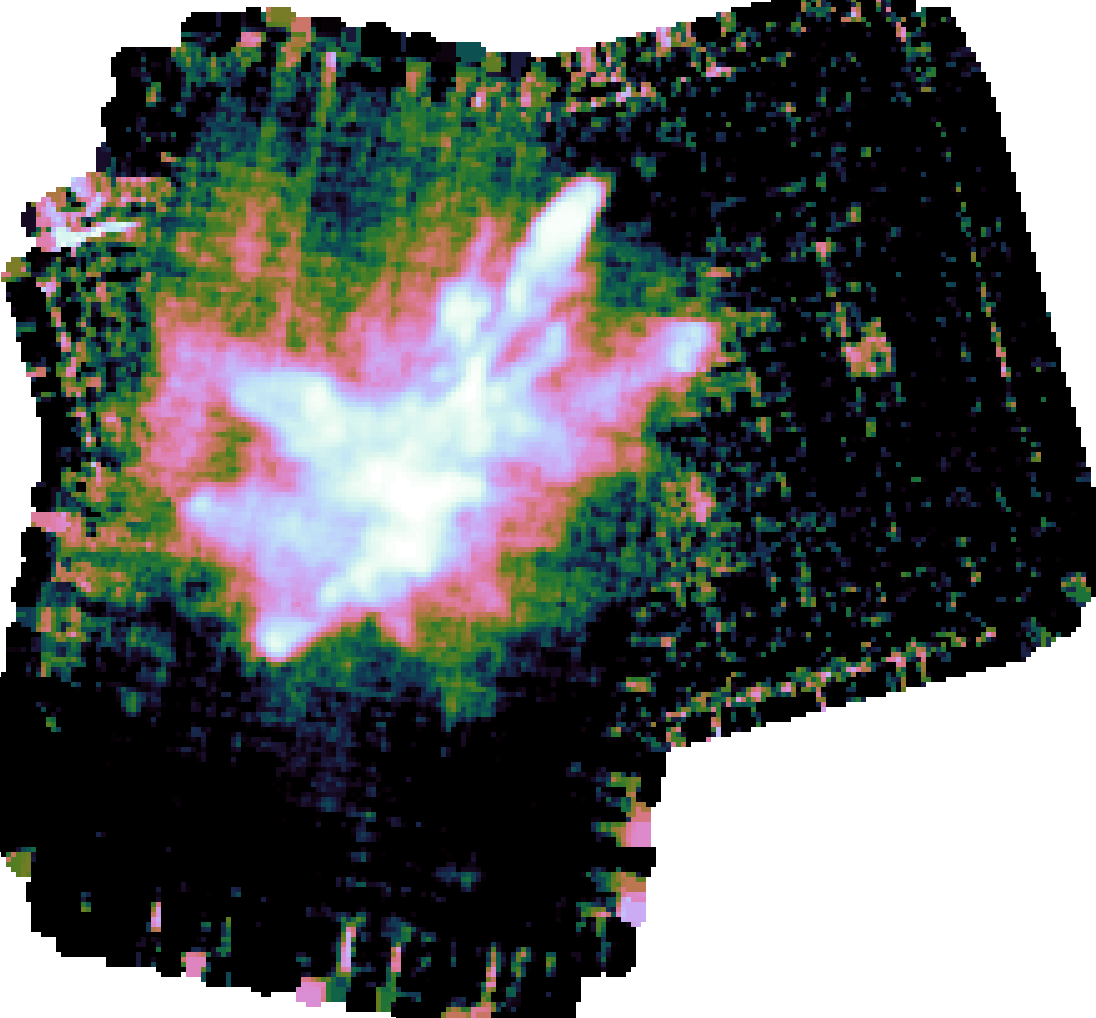
\includegraphics[width=0.46\textwidth]{integ_manual.png}
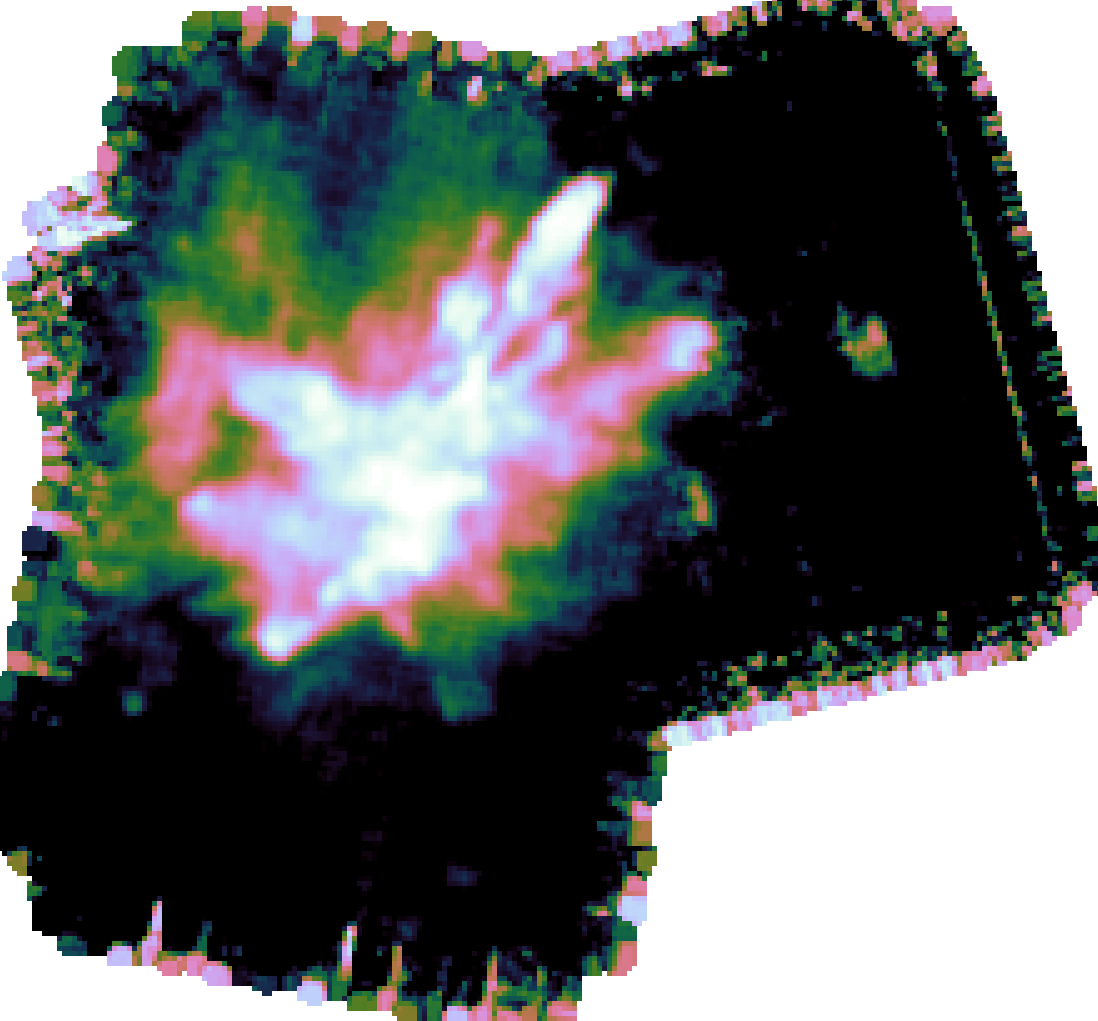
\includegraphics[width=0.46\textwidth]{integ_auto.png}
\caption{Two integrated intensity images from the same set of
  observations of Serpens from 2007 using the same display
  parameters. The left figure uses a naive sum over a significant part
  of the baseline. The right figure uses the automated baseline
  masking.}
\label{fig:integ}
\end{minipage}
\end{figure*}

Fig.\ \ref{fig:integ} compares integrated intensity images calculated
in two different ways from a single data cube generated by the
pipeline \citep[see][for details of earlier
reductions of these data]{2010MNRAS.409.1412G,2010A&A...523A..29D}. This data set
has some interference in a few spectral channels of a few receptors
that has not yet been handled by the main pipeline
processing. Neverthless, the lower image shows no sign of the grid
printing through and shows much more dynamic range than the naive
integrated intensity image.

\subsection{Removal of Bad-Baseline Spectra}



\textit{Malcolm's ADASS XXII poster and JCMT Newsletter article. Blog mentions
that we might also handle ringing in spectra.}

The bad baselines can be divided roughly into two classes:
high-frequency, high amplitude; and low frequency, lower
amplitude. The former appear mostly in single isolated spectra or in
narrow bands, but can also manifest as spiky spectra, or
weaker-amplitude striations persistent over tens of spectra.
Figure~\ref{fig:badbase:highfreq} presents the most-common forms.

\begin{figure}[!ht]
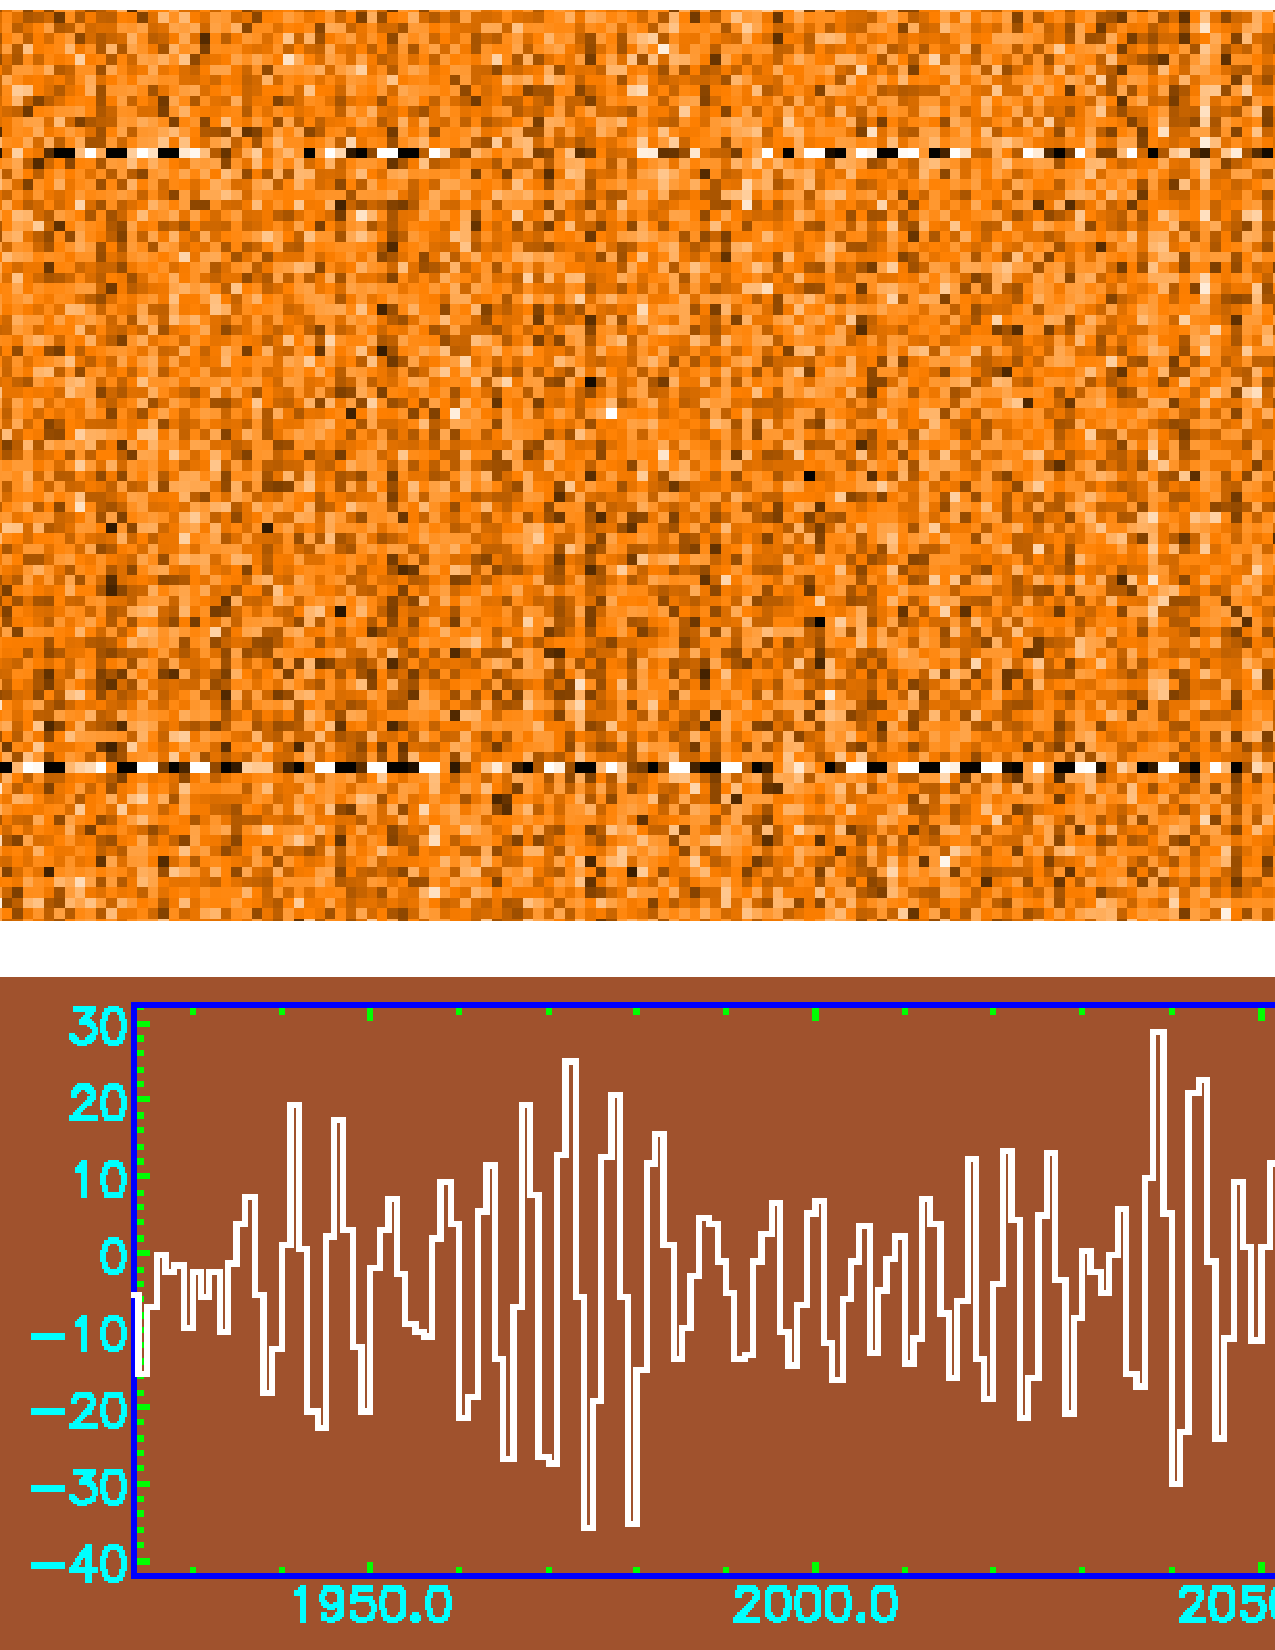
\includegraphics[width=0.23\textwidth]{P61_f1a}
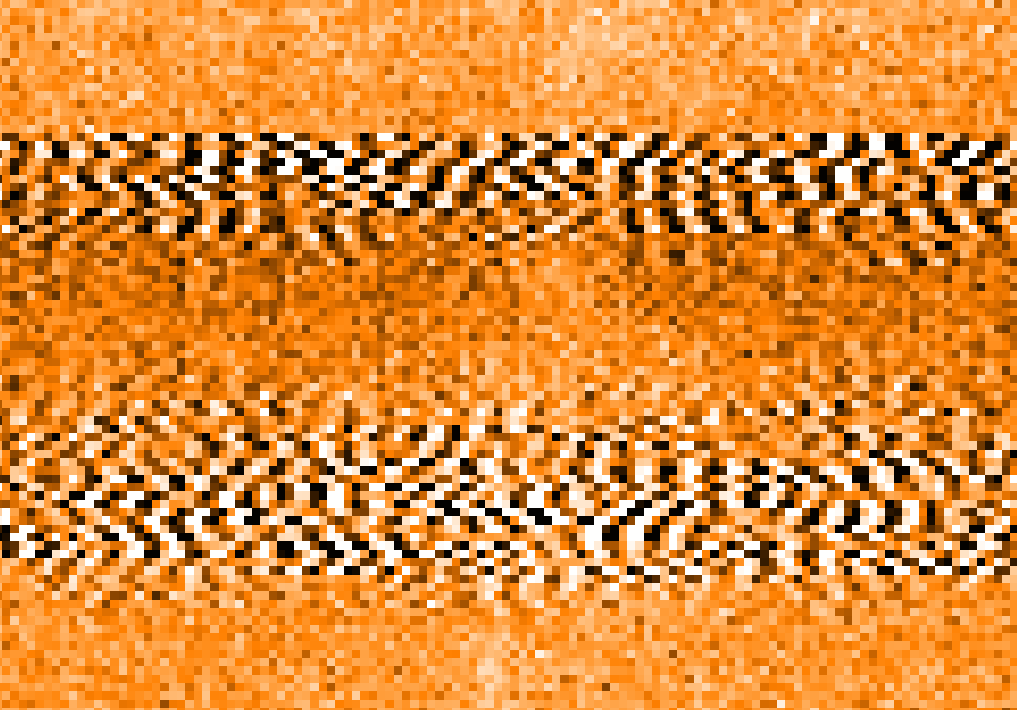
\includegraphics[width=0.23\textwidth]{P61_f1b}
\caption{Examples of high-frequency interference in spectral-time
  axes. The left panel shows high-amplitude interference affecting
  single spectra; and part of an affected spectrum plotted below. The
  amplitude dwarfs the normal signal by an order of magnitude. The
  right panel shows bands of phase-shifting interference.}
\label{fig:badbase:highfreq}
\end{figure}

The low-frequency ripples tend to occur in time-series blocks that are
often visible because of baseline drift, but can apply to all spectra
for a receptor. They have a wide range of morphologies such as
sinusoids, irregular ripples, and curved, twin headlight-like beams
that start strong but gradually pan out and fade with time.
Figure~\ref{fig:badbase:interference} displays some examples.

\begin{figure}[!ht]
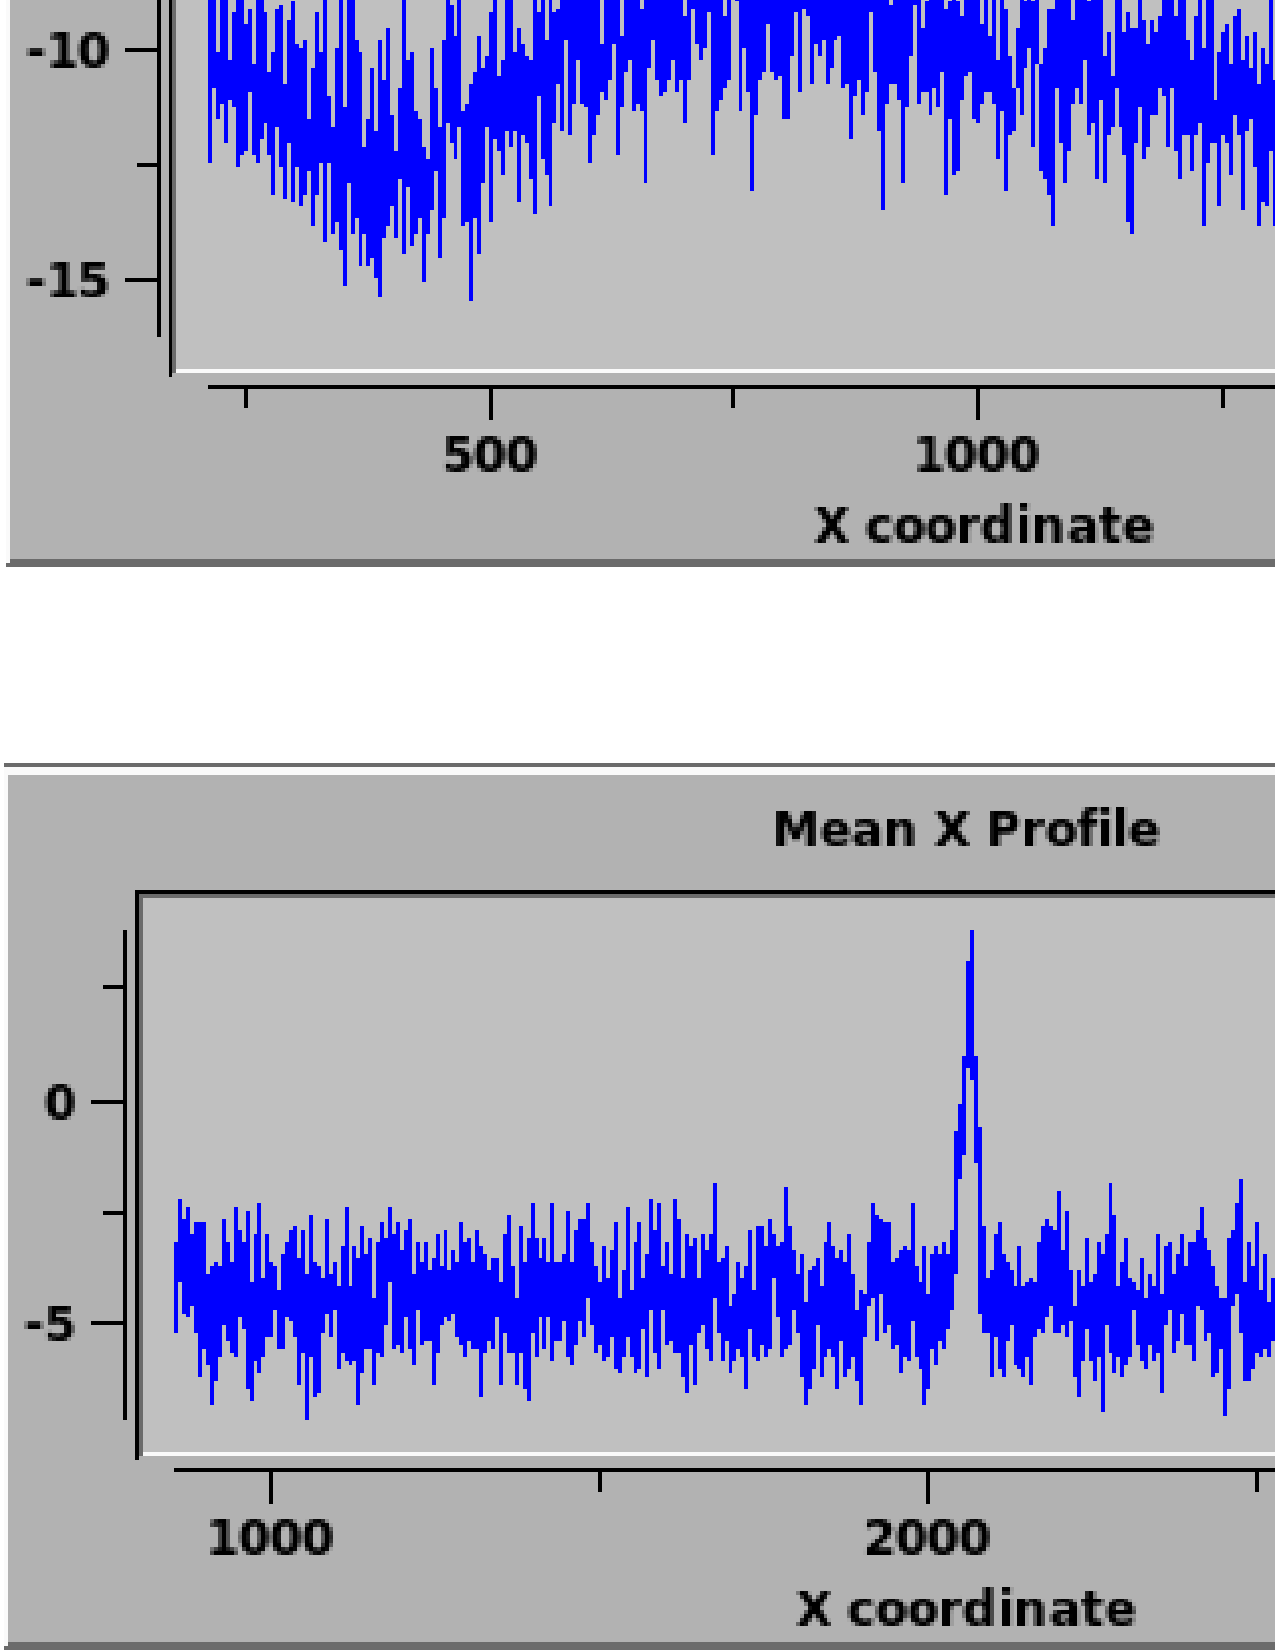
\includegraphics[width=0.23\textwidth]{P61_f2a}
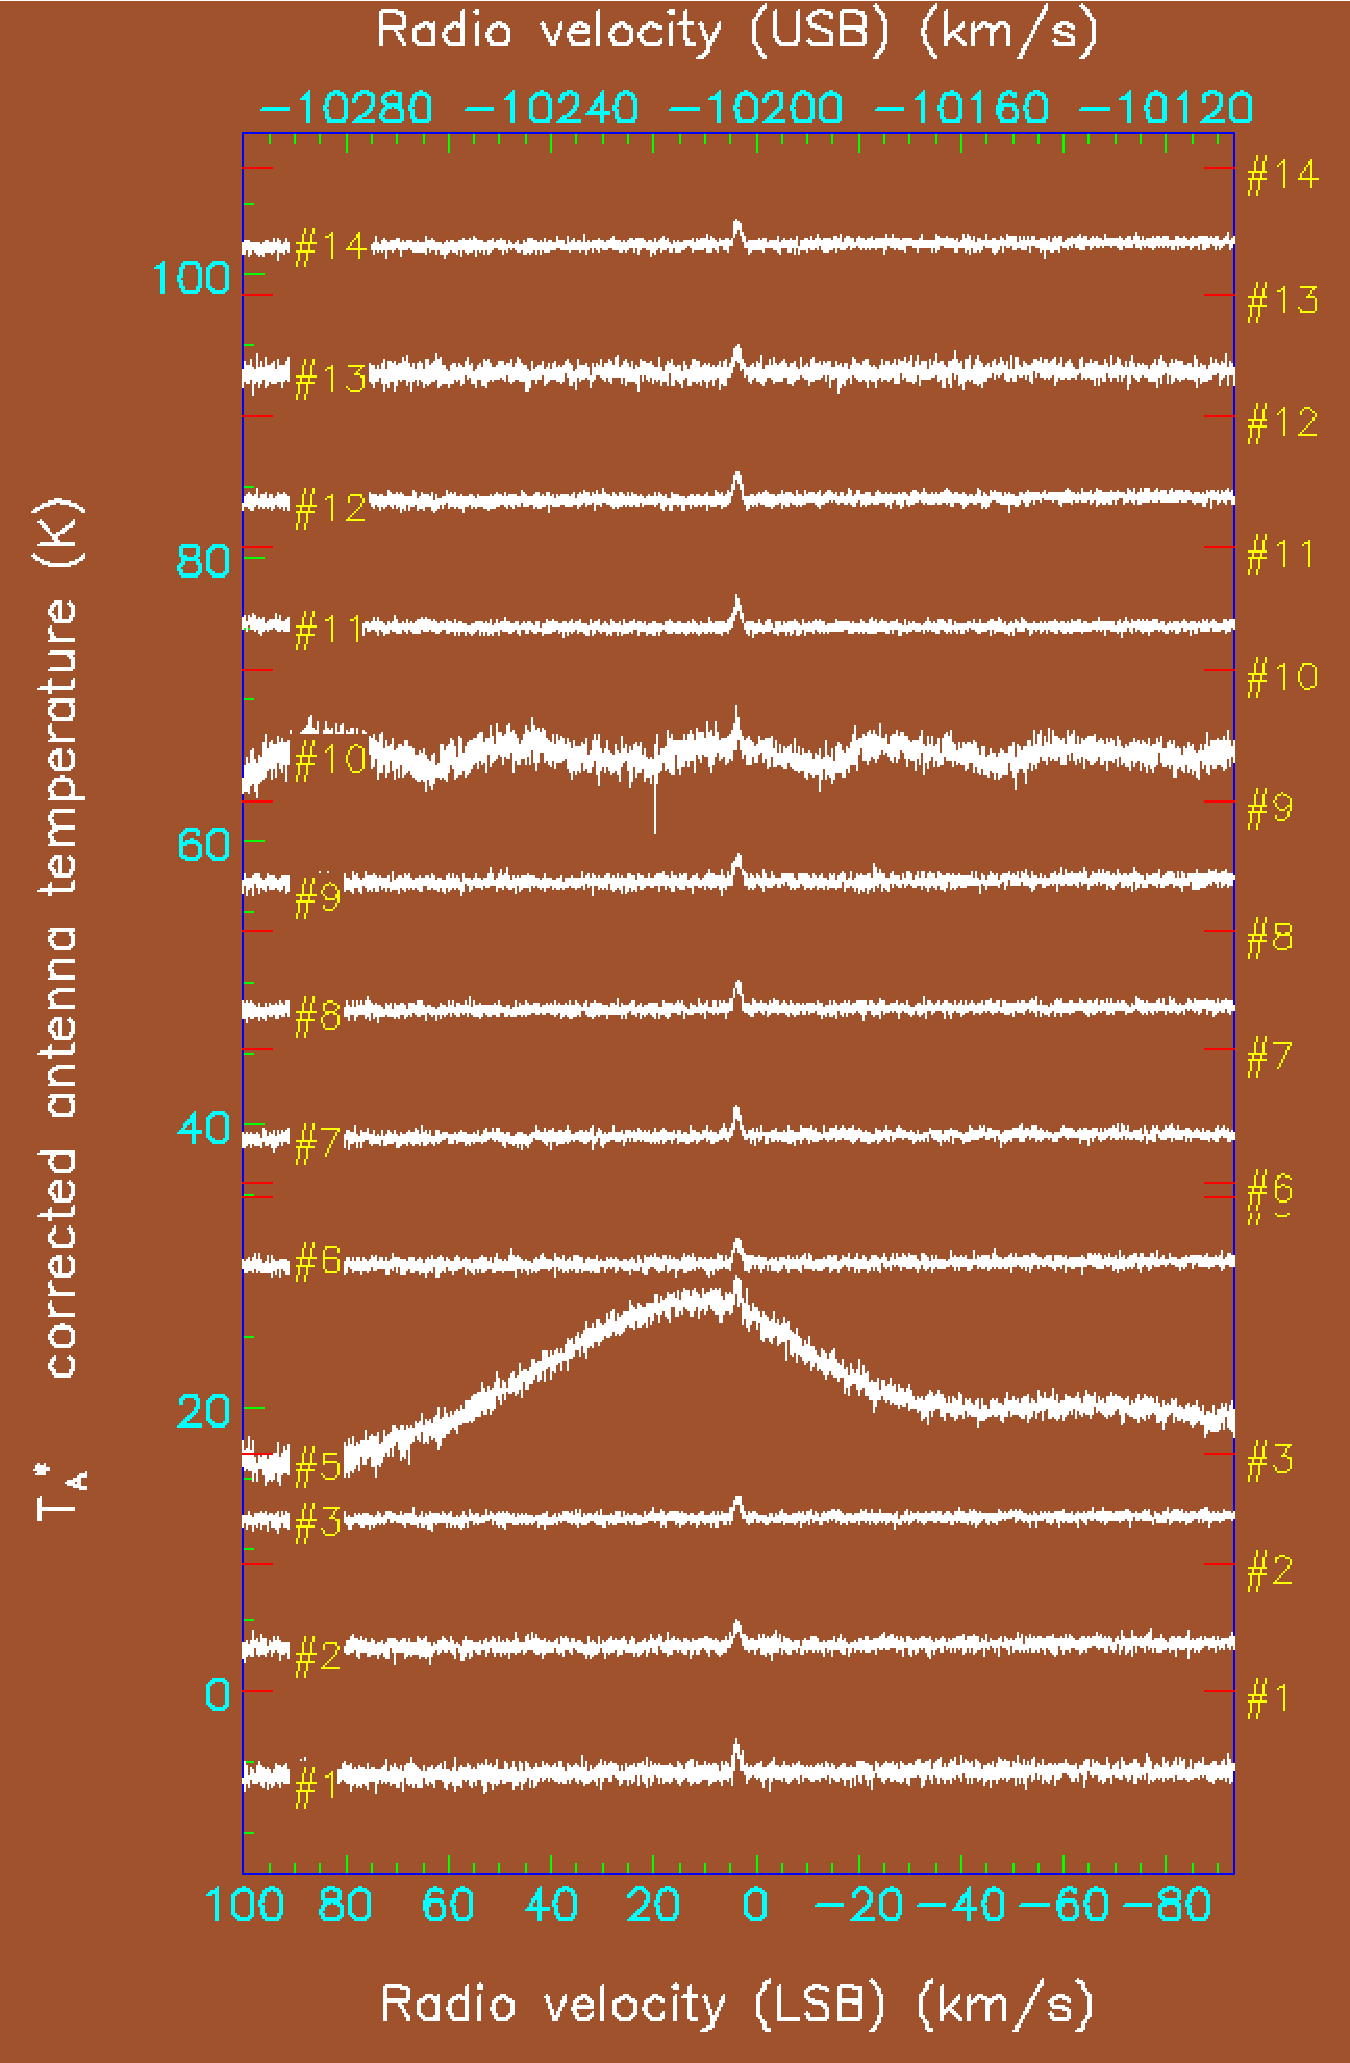
\includegraphics[width=0.23\textwidth]{P61_f2b}
\caption{Examples of low-frequency interference.  The top-left graphic
  shows a band of low-frequency oscillations; below it is the band's
  average spectrum.  The lower-left spectrum has a periodic weak
  ripple hard to detect visually.  The right panel shows time-averaged
  (clipped mean) spectra for each receptor in which the fourth and
  ninth from the bottom exhibit global non-linearity.}
\label{fig:badbase:interference}
\end{figure}

\subsubsection{Adopted solution}

The pipeline applies three steps in the quality-assurance stage:
\begin{itemize}
\item Laplacian filtering of high-frequency noise
\item non-linearity detection for individual spectra
\item global non-linearity to reject whole receptors
\end{itemize}

\subsubsection{Masking of High-Frequency Noise}

The recipe applies a one-dimensional Laplacian edge filter to all the
spectra for each receptor trimming the outer 15~\% where noise is
always present.  This approximates to a difference-of-Gaussian
filter. It next sums the rms `edginess' along the spectral axis to
form a profile through the time series.  Drifts or steps in the
profile are removed.  The final step is to eject spectra whose rms
edginess exceeds the median level by a nominated number of clipped
standard deviations.  Affected spectra are easily delineated.  An
optional second iteration removes most of the striation noise once the
pronounced edginess peaks are masked.

\subsubsection{Non-linearity Filtering}

The low-frequency rippled and wobbly baselines are addressed by
determining the non-linearity of each spectrum.  First the recipe
excludes non-baseline features that would dilute the non-linearity
signal.  These comprise a threshold to remove spikes and masking a
central region where the astronomical signal may be present. It
estimates the background level, effectively smoothing to remove
structure smaller than a nominated scale.  Next it fits linear
baselines to these and calculates the rms residuals to provide a
rectified signal.  Then it averages the signal along the spectral axis
to form a non-linearity profile through the time series for each good
receptor.

The non-linear profiles are much noisier than the summed Laplacians
and discrimination is harder.  To identify anomalous spectra the
recipe reduces the noise to obtain a smooth profile, correct for
drifts or steps in the profile.  It rejects spectra whose mean
non-linearity exceeds the mean level above a nominated number of
clipped standard deviations.  The derived standard deviation allows
for positive skewness.  It applies a mask of rejected spectra to the
input cube.

The global non-linearity test is applied last so that a block of
transient highly deviant spectra will not cause the whole receptor to
be rejected.  It operates in a similar fashion to the above.  It
diverges by determining a mean rms residual from non-linearity per
detector, from which it evaluates the median and standard deviation of
the distribution of mean rms residuals from the entire observation,
and performs iterative sigma clipping above the median to reject those
detectors whose deviations from linearity are anomalous.  There is a
tunable minimum threshold.

\subsubsection{Results}

The methods appear highly effective at cleaning the pipeline
products. It has been used to re-reduce one survey and several other
datasets. Figure~\ref{fig:badbase:results} presents an example which
had originally failed quality assurance, but now can be used for
science.

\begin{figure}
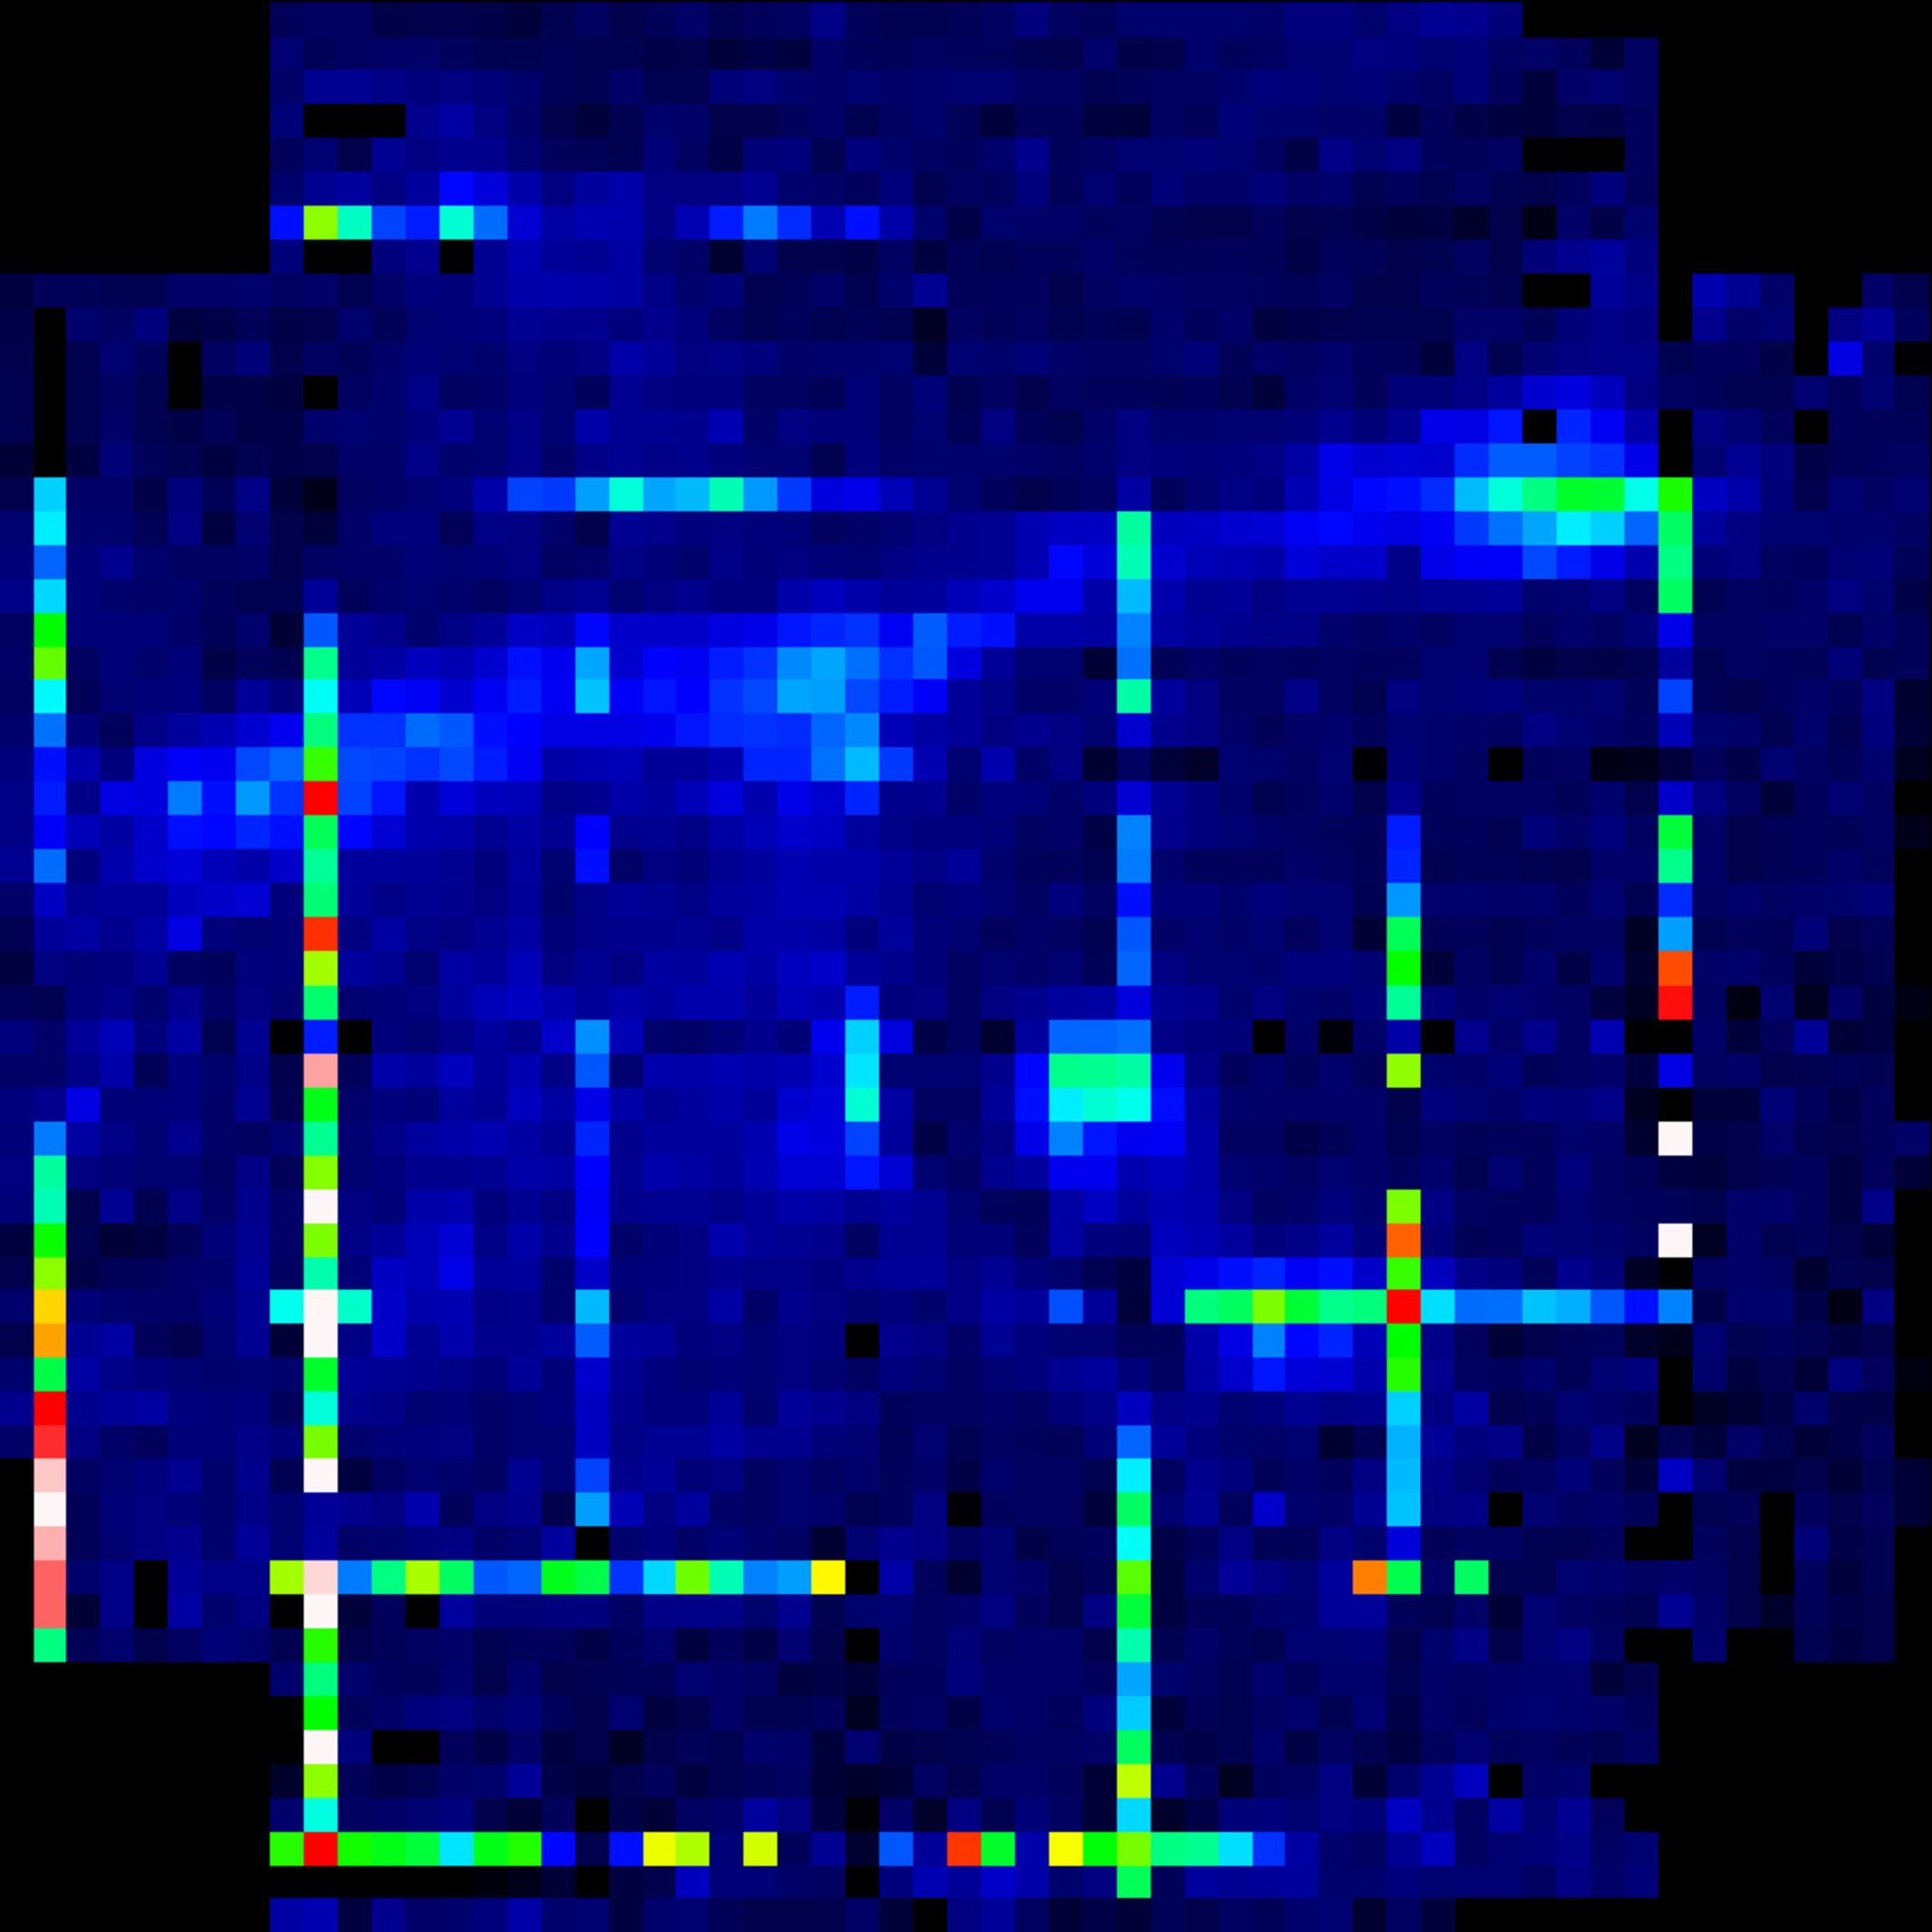
\includegraphics[width=0.23\textwidth]{P61_f3a}
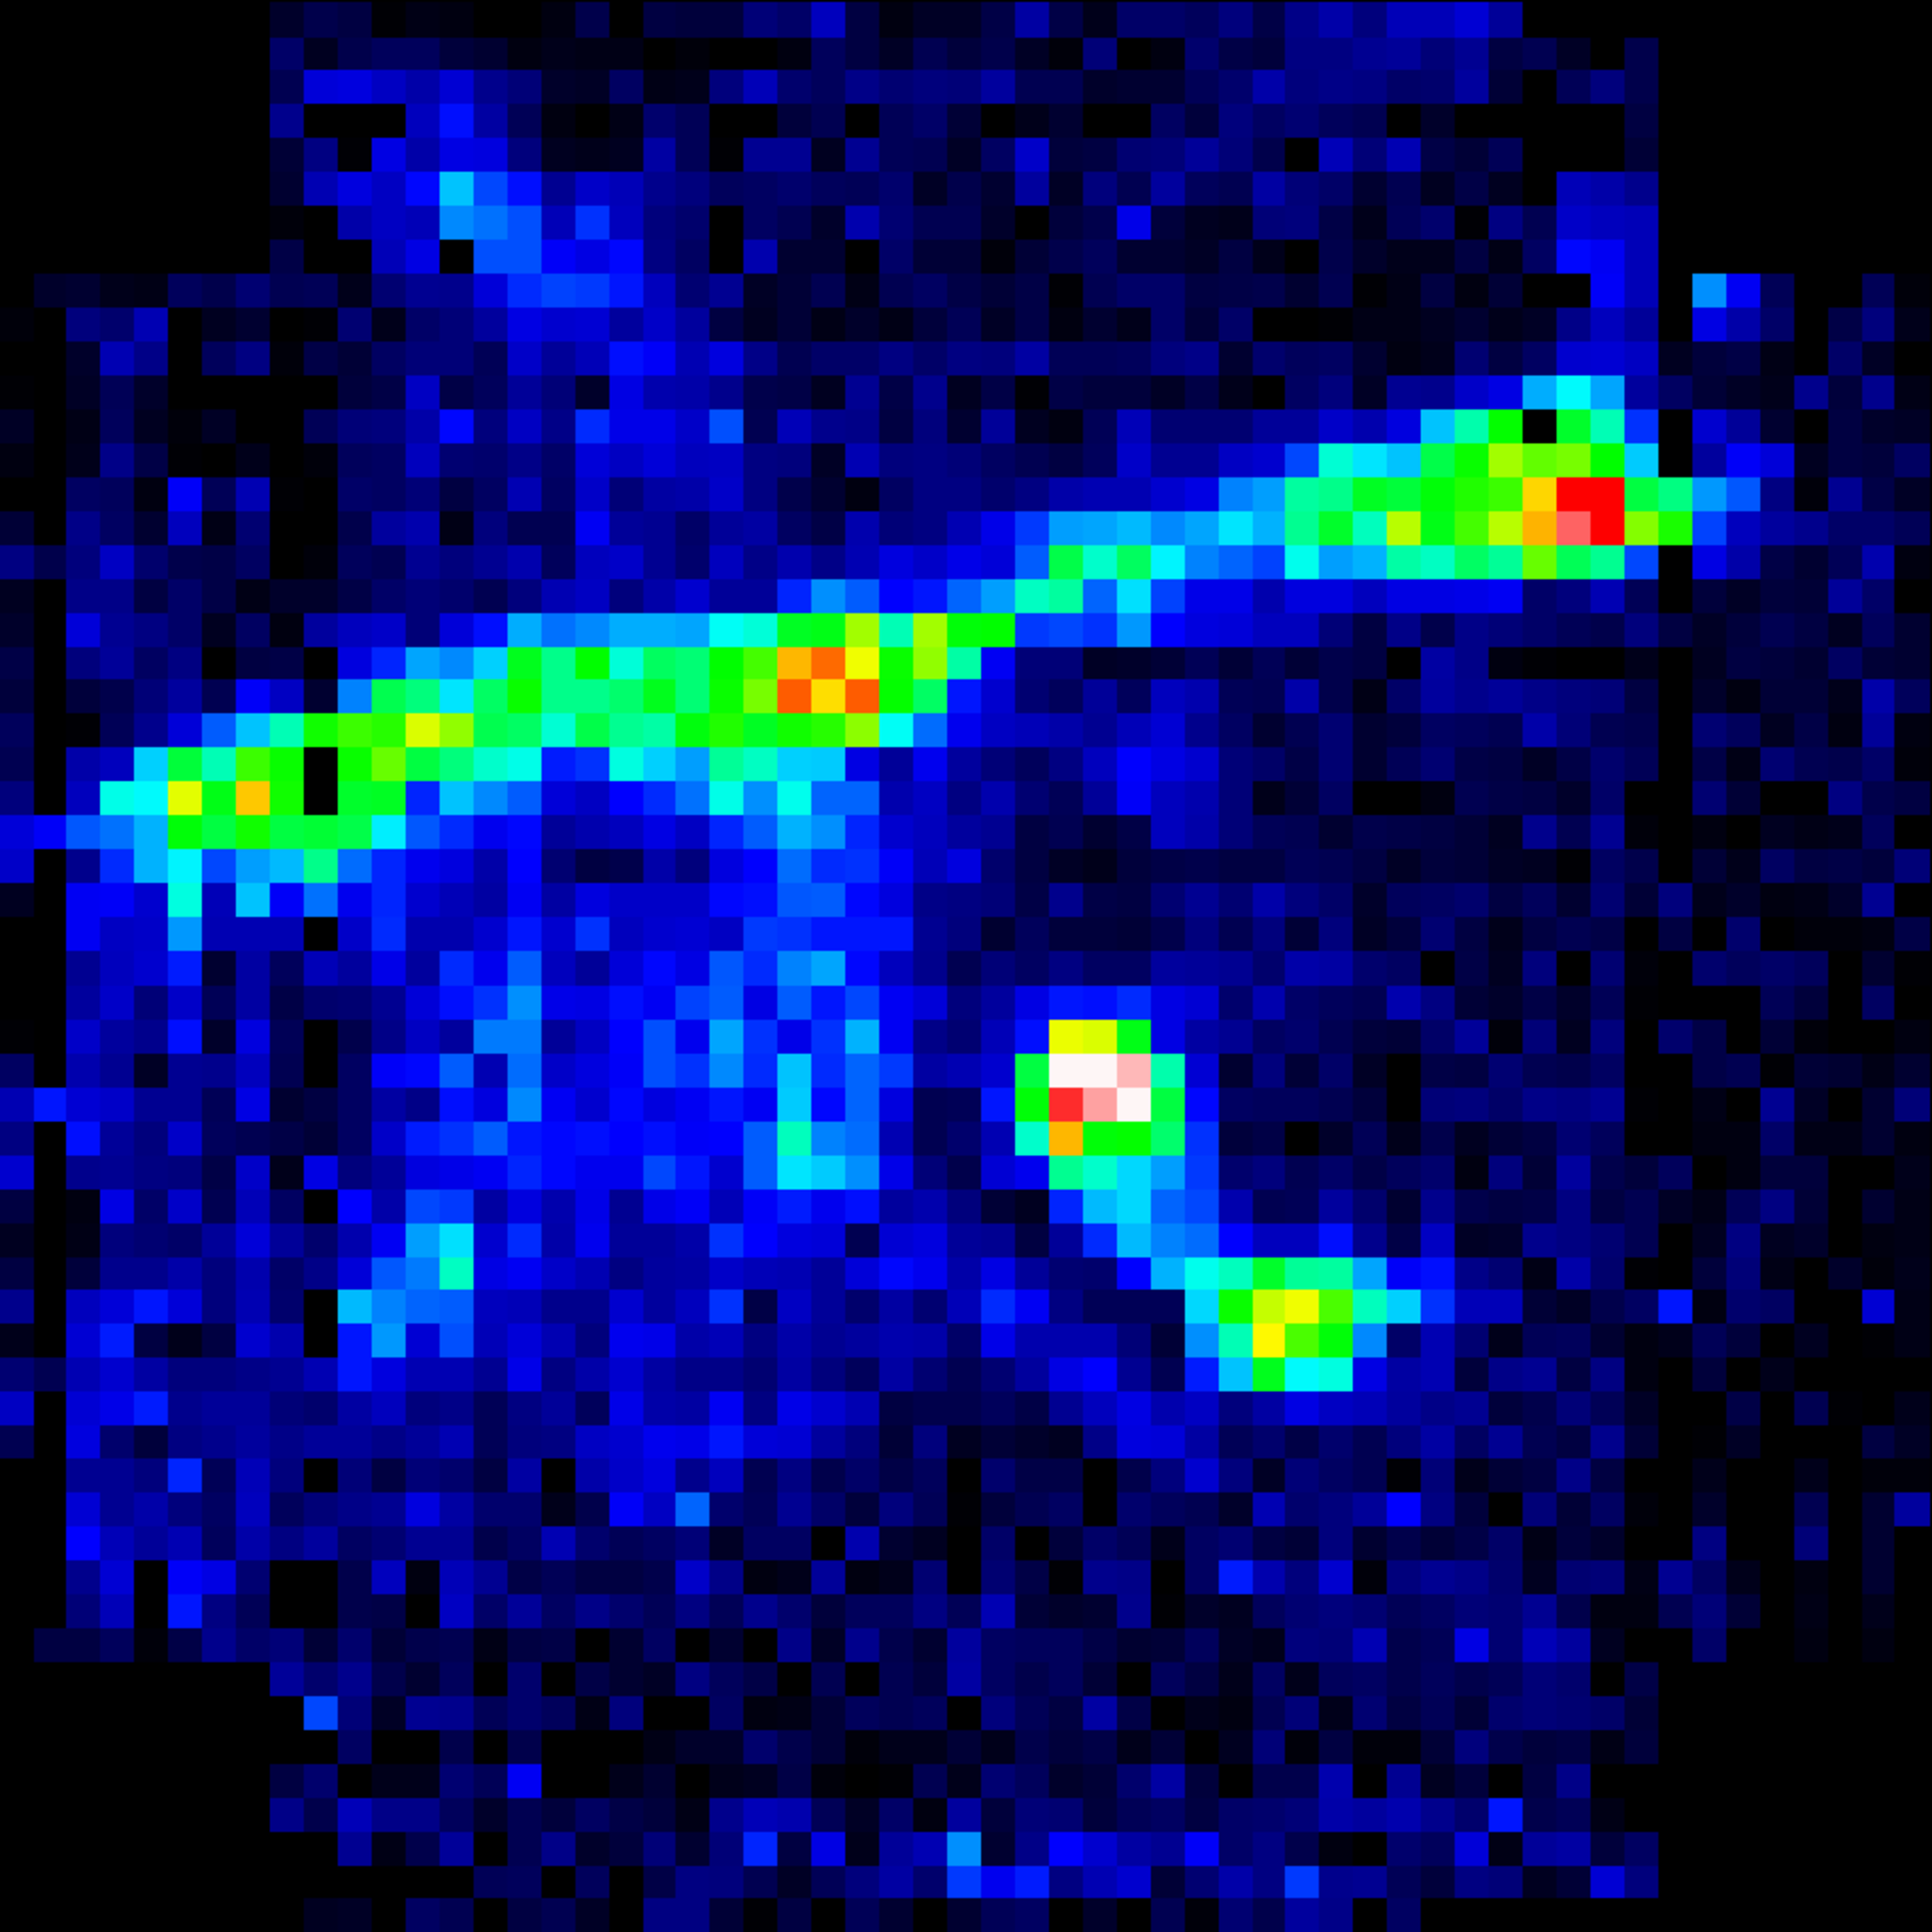
\includegraphics[width=0.23\textwidth]{P61_f3b}
\caption{Comparison of an integrated intensity map using the same
  percentile scaling.  The left panel shows a map without bad-baseline
  removal.  The right panel shows the same data processed using the
  new filters.}
\label{fig:badbase:results}
\end{figure}

\subsection{Flatfielding}

Early HARP data from 2006 seemed to have problems with the relative
calibration of the receptors. A self flatfielding algorithm was
developed that relied on the receptors on average seeing the same
signal for large scan maps of molecular clouds
\citep{2010MNRAS.401..455C} and this had some success in removing
striping from integrated intensity images.

Now discuss the pipeline implementation. Before and after flatfielding examples.

\subsection{Recipe Tuning}

The data reduction system can be configured by using recipe parameters
supplied to ORAC-DR in a file. Each recipe has its own set of
parameters that are supported and these can include options to bin up
the frequency scale, control the output grid, control any regridding
parameters and enable or disable flatfielding and bad baseline filtering.

\subsection{Quality Assurance Parameters \label{sec:qa}}

\begin{table}
  \caption{Summary of the quality assurance parameters supported by
    the pipeline. More details can be found in \citep{2008JCMTLSQA}.}
\label{tab:qa:params}
\begin{tabular}{ll}
BADPIX\_MAP  & Percentage of bad spatial pixels\\
   & in output product\\
CALINTTOL & Percentage discrepancy allowed\\
    &  in calibrator integrated intensity \\
CALPEAKTOL & Percentage discrepancy allowed\\
    & in calibrator peak\\
FLAGTSYSBAD & Percentage of data allowed \\
   & to be flagged due to T$_{sys}$\\
GOODRECEP & Number of functioning receptors\\
RESTOL & Tolerance on residuals of baseline \\
   & region after baseline subtraction\\
RESTOL\_SM & Variation of baseline residuals \\
  & over restricted range\\
RMSTOL & Consistency check comparing\\
  & T$_{sys}$ with spectrum rms\\
RMSVAR\_MAP & Percentage variation of\\
  & rms noise across map \\
RMSVAR\_RCP &  Percentage average rms receptors\\
  & are allowed to vary from each other\\
RMSVAR\_SPEC & Percentage variation of RMS\\
  & across spectrum \\
TSYSBAD &  Maximum allowable T$_{sys}$\\
TSYSMAX & Threshold for  average T$_{sys}$ \\
  & allowed for a receptor\\
TSYSVAR &  Maximum allowed variation of\\
  & T$_{sys}$ for a single receptor\\
\end{tabular}
\end{table}

The survey teams required a comprehensive set of quality assurance
testing to ensure that the data quality is consistent for the duration
of the surveys \citep{2008JCMTLSQA}. A number of QA tests were added
to the pipeline and a full list is shown in Table
\ref{tab:qa:params}. Some of these QA parameters are designed to be
run on spectral line standards observations prior to starting science
observations to determine whether the system is configured properly
and to allow the observer to decide which, if any, of the projects can
be observed next. There are also QA tests designed to look at the
time-series data and others that analyse the map/cube products.

\subsection{Alternative Recipes}

It is not possible or even desirable for a single data reduction
technique to apply to many different types of sources and science
goals. For that reason a number of different recipes are made
available and these can be chosen by the observer in the Observing
Tool, overridden later on the command-line or by using a
configuration file at the JCMT Science Archive.

\subsubsection{Gradient}

This is the standard recipe optimized for nearby molecular clouds with
relatively narrow lines where there can be a velocity gradient across
the cloud. This velocity gradient is a major motivation for the
automated detection of baseline regions as it allows you to maximize
the baseline region rather than supplying a simple range that
encompasses all the data.

\subsubsection{Broad line}

Nearby galaxies have broad lines of many km/s so this recipe is tuned
to be less aggressive for automatic baseline subtraction than the
standard recipe that is deisgned for nearby molecular clouds. An early
form of this recipe, in the form of a standalone script, was used for
the initial Nearby Galaxy Survey data release and is documented in
\citet{2010ApJ...714..571W}.

\subsubsection{Line Forest}

Some transitions are very close together, for example methanol, and
different techniques are required for handling the automated basline
subtraction.

\textit{Actually, the recipe itself implies that it's more or less the
  same as the standard gradient recipe}

\subsubsection{Continuum}

For continuum observations, such as planets, baseline subtraction
should not be done.

\section{Processing of Historical JCMT Data}

Until ACSIS was delivered in 2005, heterodyne data were taken with a
variety of backend systems including the Acousto-Optical Spectrometer
(AOSC) and the Dutch Autocorrelation Spectrometer (DAS)
\citep{1986SPIE..598..134B}. These backends wrote data in the
Global Section Data (GSD) format \citep[e.g.][]{GSD1999} which was
understood by the SPECX data reduction package. To ensure that as much
of this historical data as possible is made available to the community
in a useable format we have developed an extension to the SMURF
package called \textsc{gsd2acsis} that converts the legacy data to the
newer ACSIS data format (which is based on the Starlink NDF format
\citep{NDF,1988STARB...2...11C,P91_adassxxiii}). This enables the legacy data to be re-processed using
the modern data reduction pipeline and automatically leads to these
products being easily available from the JCMT Science Archive.

The main difficulty in supporting legacy data in the pipeline related
to the DAS splitting the bandwidth into many overlapping
subbands. ACSIS data only ever had included two subbands for hybrid
mode observations and so the subband merging algorithm had to be
extended to support arbitrary numbers of subbands. Additionally, the
historical data are dominated by single-receptor instruments and most
observations generated relatively few spectra, and few repeats of the
same area of sky (depth in the first pass was preferred over short
integration times but many repeats). This sometimes
restricts the benefits that can be obtained by using a pipeline
designed for focal plane arrays.

We tested the pipeline on one of the largest data sets from the
historical era. Observations of the Horsehead nebula were an
observatory backup project from 1995 to 1997. The $^{13}$CO
$J=2\rightarrow 1$ component of the project consisted of approximately
14,000 spectra from 154 observations spread over 12 nights using the
single receptor receiver RxA2 \citep{1992IJIMW..13..647D}. Reducing
the data with SPECX was an involved process and preliminary results
were presented in \citet{2001AAS...19915601S}. For this test the GSD data were
downloaded from the CADC and converted to ACSIS format.

For these observations there were two major difficulties. The data
were taken in raster scan mode with over-sampling in the scan
direction (to prevent beam-smearing) and Nyquist sampling between
rows. For the JCMT beam at this frequency this corresponds for
5\,arcsec and 10\,arcsec spacing. The pipeline has not been optimized
for this observing scheme although it correctly selected a 5\,arcsec
pixel size. This meant that half of the map contained bad pixels and
so an additional interpolation routine was required before the final
integrated intensity image could be calculated. A consequence of the
large number of flagged pixels in the map was that the quality
assurance test associated with bad pixel map fraction had to be
relaxed significantly.

For some of the observations a bad reference position had been chosen,
which leads to absorption features in some spectra. These data were
used in the manual reduction because a long observation was taken on
this reference position along with a new ``off'' position and the
spectra corrected. Doing this in an automated fashion is difficult
without more investigation into the related observations as GSD data
did not record the location of the reference position in the
header. For the purposes of the test these observations were not used.

The results can be seen in Fig.\ \ref{fig:hhcmp}. The SPECX ``manual''
reduction does look better than the automated reduction, especially in
the region in the north east where some contamination still seems to
be present. It seems feasible to assume that some of this can be
improved upon by writing recipes specifically targeted at legacy data
but the proof of concept is encouraging.

\begin{figure*}
\begin{minipage}{\textwidth}
\centering
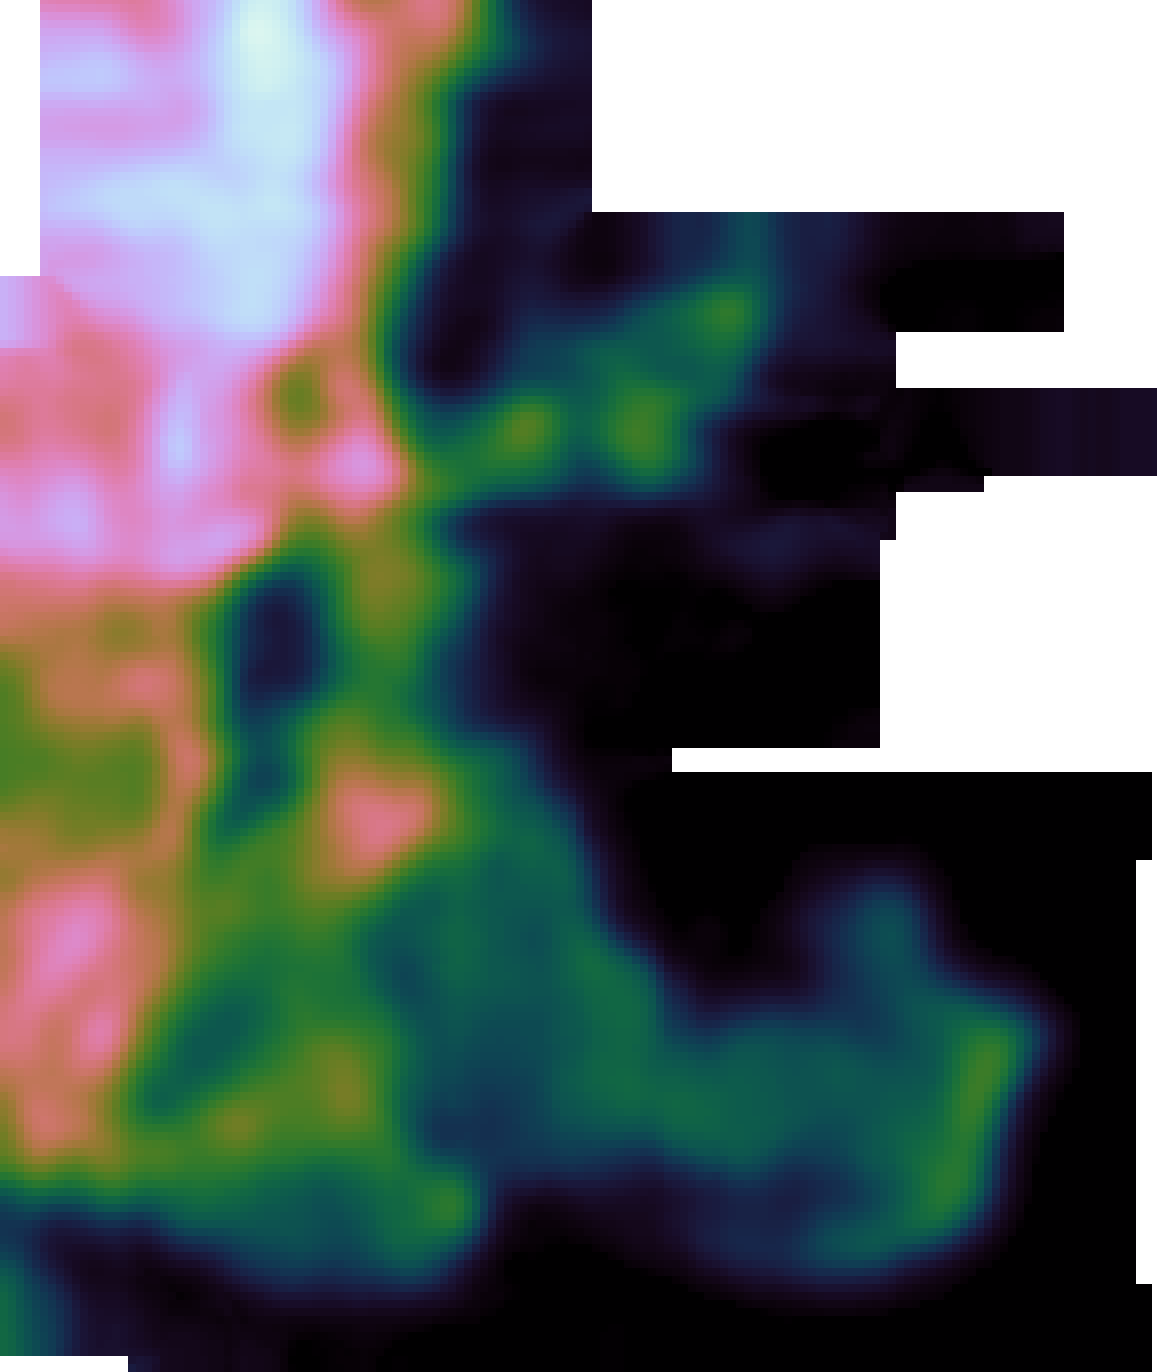
\includegraphics[width=0.46\textwidth]{horsehead-specx}
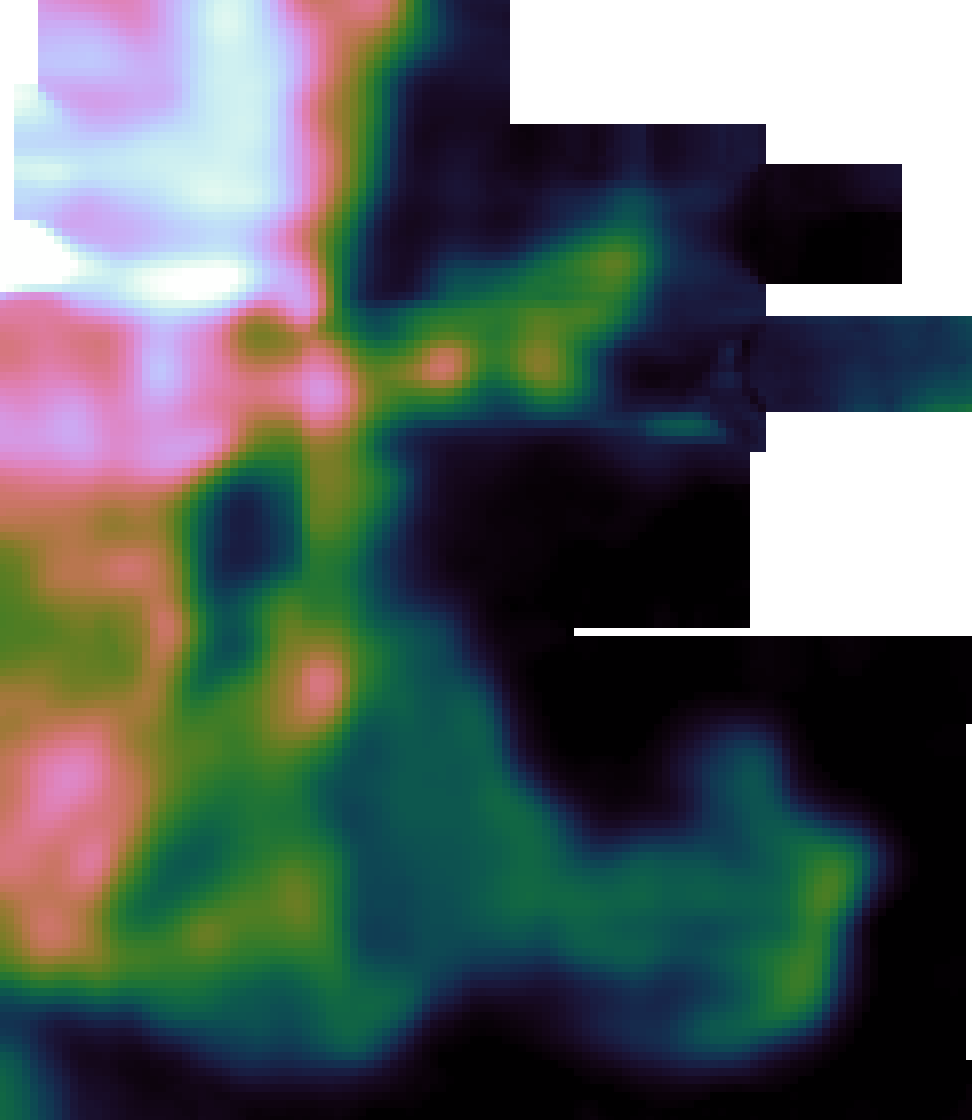
\includegraphics[width=0.46\textwidth]{horsehead-pipeline}
\caption{Left is an integrated intensity image created from
  a cube made interactively using SPECX. Right is an
  integrated intensity image made from a pipeline reduction of the
  same raw data. Intensity scales are 0 to 35 K\,km/s.}
\label{fig:hhcmp}
\end{minipage}
\end{figure*}

\section{Conclusion}

With many thousands of spectra from a single observation it is
impractical to examine every spectrum manually. The data reduction
scheme described here is used continually at the JCMT Science Archive
\citep{2011ASPC..442..203E} for daily and project processing and the
tuned recipes are now generating the primary products from the
heterodyne part of the Gould's Belt JCMT Legacy Survey
\citep{2007PASP..119..855W} and also the CO High Resolution Survey
(COHRS) from the JCMT \citep{2013ApJS..209....8D}.

The iterative pipeline processing described in this paper demonstrates
the possibilities for advanced heterodyne cube reconstruction if we
begin to use techniques more akin to those used by iterative
map-makers for bolometer cameras
\citep[e.g.][]{2013MNRAS.430.2545C}. The next step is to explicitly
embrace such techniques, building up explicit models of the
astronomical emission and baselines and enhance this to have models
involving knowledge of which detectors have related local oscillators
and which detectors come from the same backend hardware. This latter
facility may be important as more and more detectors are added to
focal plane arrays and would be similar to dealing with readout issues
of bolometer arrays.

\textit{At one point Per was mentioning that Kriging would be a useful
  option in makecube for doing an optimal unbiased linear
  interpolation method. I wonder if we should mention it here as an
  option for future work. In terms of ``Bolometer map-maker'' we do
  have the problem that our sampling is much more course than these
  big bolometer cameras so I'm not sure whether we need to point that
  out.}

\section{Acknowledgments}

The James Clerk Maxwell Telescope is operated by the Joint Astronomy
Centre on behalf of the Science and Technology Facilities Council of
the United Kingdom, the National Research Council of Canada, and
(until 31 March 2013) the Netherlands Organisation for Scientific
Research. We thank the many JCMT support scientists and survey
scientists who have tested the pipeline. In particular we thank
Jessica Dempsey, Holly Thomas, Jan Wouterloot, Jane Buckle and
Jennifer Hatchell. We would also like to thank Jennifer Balfour and
Vincent Tilanus for their work on \textsc{gsd2acsis}. We thank
G.~Sandell for providing us with the SPECX reductions of the Horsehead
Nebula. This research used the facilities of the Canadian Astronomy
Data Centre operated by the National Research Council of Canada with
the support of the Canadian Space Agency.

This work was built on the Starlink Software Collection, which was
developed by the Starlink Project until 2005
\citep{1982QJRAS..23..485D,2005ASPC..347...22D,2008ASPC..394..650C}
and then opened up to the community. The source code for the Starlink
software (ascl:1110.012) and ORAC-DR (ascl:1310.001) is open-source and is
available on github at
\htmladdnormallink{https://github.com/Starlink}.

%% The Appendices part is started with the command \appendix;
%% appendix sections are then done as normal sections
%% \appendix

%% \section{}
%% \label{}

%% References
%%
%% Following citation commands can be used in the body text:
%%
%%  \citet{key}  ==>>  Jones et al. (1990)
%%  \citep{key}  ==>>  (Jones et al., 1990)
%%
%% Multiple citations as normal:
%% \citep{key1,key2}         ==>> (Jones et al., 1990; Smith, 1989)
%%                            or  (Jones et al., 1990, 1991)
%%                            or  (Jones et al., 1990a,b)
%% \cite{key} is the equivalent of \citet{key} in author-year mode
%%
%% Full author lists may be forced with \citet* or \citep*, e.g.
%%   \citep*{key}            ==>> (Jones, Baker, and Williams, 1990)
%%
%% Optional notes as:
%%   \citep[chap. 2]{key}    ==>> (Jones et al., 1990, chap. 2)
%%   \citep[e.g.,][]{key}    ==>> (e.g., Jones et al., 1990)
%%   \citep[see][pg. 34]{key}==>> (see Jones et al., 1990, pg. 34)
%%  (Note: in standard LaTeX, only one note is allowed, after the ref.
%%   Here, one note is like the standard, two make pre- and post-notes.)
%%
%%   \citealt{key}          ==>> Jones et al. 1990
%%   \citealt*{key}         ==>> Jones, Baker, and Williams 1990
%%   \citealp{key}          ==>> Jones et al., 1990
%%   \citealp*{key}         ==>> Jones, Baker, and Williams, 1990
%%
%% Additional citation possibilities
%%   \citeauthor{key}       ==>> Jones et al.
%%   \citeauthor*{key}      ==>> Jones, Baker, and Williams
%%   \citeyear{key}         ==>> 1990
%%   \citeyearpar{key}      ==>> (1990)
%%   \citetext{priv. comm.} ==>> (priv. comm.)
%%   \citenum{key}          ==>> 11 [non-superscripted]
%% Note: full author lists depends on whether the bib style supports them;
%%       if not, the abbreviated list is printed even when full requested.
%%
%% For names like della Robbia at the start of a sentence, use
%%   \Citet{dRob98}         ==>> Della Robbia (1998)
%%   \Citep{dRob98}         ==>> (Della Robbia, 1998)
%%   \Citeauthor{dRob98}    ==>> Della Robbia


%% References with bibTeX database:

\bibliographystyle{model2-names-astronomy}
\bibliography{acsisdr}

%% Authors are advised to submit their bibtex database files. They are
%% requested to list a bibtex style file in the manuscript if they do
%% not want to use model2-names.bst.

%% References without bibTeX database:

% \begin{thebibliography}{00}

%% \bibitem must have one of the following forms:
%%   \bibitem[Jones et al.(1990)]{key}...
%%   \bibitem[Jones et al.(1990)Jones, Baker, and Williams]{key}...
%%   \bibitem[Jones et al., 1990]{key}...
%%   \bibitem[\protect\citeauthoryear{Jones, Baker, and Williams}{Jones
%%       et al.}{1990}]{key}...
%%   \bibitem[\protect\citeauthoryear{Jones et al.}{1990}]{key}...
%%   \bibitem[\protect\astroncite{Jones et al.}{1990}]{key}...
%%   \bibitem[\protect\citename{Jones et al., }1990]{key}...
%%   \harvarditem[Jones et al.]{Jones, Baker, and Williams}{1990}{key}...
%%

% \bibitem[ ()]{}

% \end{thebibliography}

\end{document}

%%
%% End of file `elsarticle-template-2-harv.tex'.
